\specialchapter{HISTORICAL NOTE (CHAPTERS IV, V AND VI)}

(N.B. - The roman numerals in parentheses refer to the bibliography at the end of this note.)

The groups considered in these chapters appeared in connection with various questions of Geometry. Analysis and the Theory of Lie groups, sometimes in the form of permutation groups and sometimes in the form of groups of displacements in euclidean or hyperbolic geometry, and these various points of view have been unified only recently.

The historical roots of the theory are substantially earlier than the introduction of the concept of a group: indeed, they are found in the studies of the ``regularity'' or ``symmetries'' of geometrical figures, and notably in the determination of the regular polygons and polyhedra (which certainly goes back to the Pythagoreans), which constitutes the crowning achievement of the Elements of Euclid and one of the most admirable creations of the Greek genius. Later, notably with the Arab authors of the high Middle Ages, and then with Kepler, the beginnings of the mathematical theory of regular ``tilings'' of the plane or the sphere by (not necessarily regular) congruent polygons appear; this is undoubtedly related to the various types of decoration devised by the ancient and Arab civilisations (which can properly be considered as an authentic part of the mathematics developed by these civilisations (XII)).

Around 1830-1840, studies in crystallography (Hessel, Bravais, Möbius) lead to the consideration of a problem that is actually the determination of the finite groups of displacements in euclidean space of 3 dimensions, although the authors quoted above do not yet use the language of group theory; that does not really come into use until about 1860, and it is in the context of the classification of groups that Jordan, in 1869 (VI), determines the discrete groups of orientation-preserving displacements of \(\mathbf{R}^3\) (and, more generally, the closed subgroups of the group of orientation-preserving displacements).

This stream of ideas develops in many directions until the final years of the 19th century. The most significant of these developments are the following:

\begin{enumerate}
\def\labelenumi{\arabic{enumi}.}
\item
  Continuing a trend that appears very early in the theory of finite groups, ``presentations'' of finite groups of displacements by generators and relations of a simple type are sought. Thus, Hamilton, in 1856 (V), proves that the finite groups of rotations of euclidean space \(\mathbf{R}^3\) are generated by two generators S.T satisfying the relations \(S^p = T^q = (ST)^3 = 1\) for appropriate values of \(p\) and \(q\) .
\item
  Discrete groups of displacements may or may not contain reflections. In 1852. Möbius essentially determines the finite groups of displacements in spherical geometry generated by reflections (which is equivalent to the same problem for finite groups of euclidean displacements of \(\mathbf{R}^3\) ): he finds that, with the exception of the cyclic groups, such a group has as fundamental domain a spherical triangle with sides of the form \(\pi / p, \pi / q, \pi / r\) , where \(p, q, r\) are three integers \(>1\) such that \(\frac{1}{p} + \frac{1}{q} + \frac{1}{r} > 1\) (III) (cf.~Chap. V. §4, Exerc. 4). He also notices that these groups contain all the finite groups of displacements as subgroups.
\item
  The latter developments are extended into a new area when the study of ``tilings'' of the complex plane or of the half-plane by means of figures bounded by circular arcs begins, following the work of Riemann and Schwarz on hypergeometric functions and conformal representations: Klein and Poincaré make it the foundation of the theory of ``automorphic functions'' and recognise in it (for the case of circular arcs orthogonal to a fixed straight line) a problem equivalent to the determination of the discrete groups of displacements of the non-euclidean hyperbolic plane (identified with the ``Poincaré half-plane'') (X).
\item
  The notions of regular polyhedron and of the tiling of \(R^{3}\) by such polyhedra are extended to all the euclidean spaces \(R^{n}\) by Schlättli, in work that goes back to about 1850, but which was only published much later and which was ignored for a long time (IV); he determines completely the regular ``polytopes'' in each \(R^{n}\) , the group of displacements leaving invariant such a polytope, and a fundamental domain of this group which, as in the case n = 3 studied by Möbius, is a ``chamber'' whose projection on the sphere \(S_{n-1}\) is a spherical simplex. However, he does not take up the inverse problem of determining the finite groups of displacements generated by reflections in \(R^{n}\) ; this problem will only be solved much later, by Goursat for n = 4 (VII), and for arbitrary n in the work of E. Cartan (IX f)) and Coxeter (XIV), to which we shall return later.
\end{enumerate}

With the work of Killing and of E. Cartan on Lie groups, a new stream of ideas begins around 1890 that will develop for a long period without links to the preceding work. In the study of Killing (VIII) and Cartan (IX \(a\) ) of the structure of complex semisimple Lie algebras, certain linear forms \(\omega_{\alpha}\) on a ``Cartan subalgebra'' \(\mathfrak{h}\) of such a Lie algebra \(\mathfrak{g}\) immediately play a basic role; they are the ``roots'' relative to \(\mathfrak{h}\) , so called because they appear as the roots of the characteristic equation \(\det(\operatorname{ad}_{\mathfrak{g}}(x)-T)=0\) , considered as functions of \(x\in\mathfrak{h}\) . The properties of these ``roots'' established by Killing and Cartan amount to the assertion that, in the language of Chap. VI, they form a ``reduced root system'' (cf.~Chap. VI. §1. no. 4); they then show that the classification of the complex semisimple Lie algebras reduces to that of the associated ``root systems'', which itself reduces to the determination of certain matrices with integer coefficients (later called ``Cartan matrices'': cf.~Chap. VI. § 1, no. 5). Killing and Cartan also show the existence, for every root \(\omega_{\alpha}\) , of an involutive permutation \(S_{\alpha}\) of the set of roots \(^{8}\) ; they use in an essential way the transformation \(C = S_{\alpha_1}S_{\alpha_2} \ldots S_{\alpha_l}\) , the product of the permutations associated with \(l\) roots forming a fundamental system (a transformation today called a ``Coxeter transformation''); they even extend this permutation to a linear transformation of the vector space generated by the fundamental roots \(\omega_{\alpha_i}\) ( \(1 \leqslant i \leqslant l\) ), and study its eigenvalues ((VIII. II), p.~20; (IX \(a\) )). p.~58). But neither Killing, nor Cartan initially seem to have thought of considering the group \(\mathcal{G}'\) generated by the \(S_{\alpha}\) ; and when Cartan, a little later (IX \(b\) )), determines the Galois group \(\mathcal{G}\) of the characteristic equation

\[
\det (\operatorname{ad} _ {\mathfrak {g}} (x) - \mathrm{T}) = 0
\]

of a ``general element'' \(x \in h\) , he studies it initially without bringing in the \(S_{\alpha}\) ; thirty years later, under the influence of H. Weyl, he proves (IX c)) that \(G'\) is a normal subgroup of G and determines in all cases the structure of the quotient group \(G/G'\) which (for a simple Lie algebra g) is of order 1 or 2, except for type \(D_{4}\) where it is isomorphic to \(S_{3}\) ; at the same time he interprets \(G'\) as the group induced by the inner automorphisms of a complex semisimple Lie algebra leaving fixed a Cartan subalgebra \(^{9}\) .

The work of H. Weyl, to which we have just alluded, inaugurated the geometric interpretation of the group \(G'\) (since called the ``Weyl group'' of g); he had the idea of considering the \(S_{\alpha}\) as reflections in the vector space of linear forms on h, in the same way as Killing and Cartan had done for the transformation C. It is also in the memoir (XIII) of H. Weyl that the fundamental domain of the ``affine Weyl group'' appears (but without the link to the ``Weyl group'' \(G'\) being clearly indicated); Weyl uses it to prove that the fundamental group of a compact semisimple group is finite, a crucial point in his proof of the complete reducibility of the linear representations of a complex semisimple Lie algebra. A little later, E. Cartan completes the synthesis of the global points of view of H. Weyl, of his own theory of real or complex semisimple Lie algebras, and of the theory of riemannian symmetric spaces that he was then constructing. In the memoir (IX d), he completes the determination of the fundamental polytopes of the Weyl group and of the affine Weyl group, and introduces the systems of weights and radical weights (Chap. VI, §1, no. 9); in (IX c)) he extends this discussion to symmetric spaces, and notably encounters the first examples of non-reduced root systems (Chap. VI, §4, no. 1). Finally, the article (IX f)) gives the first proof that every irreducible finite group generated by reflections in \(R^{n}\) has a fundamental domain whose projection onto \(S_{n-1}\) is a spherical simplex; it is also in this work that he proves the uniqueness of the highest root (for an arbitrary lexicographic ordering on the root system) by geometrical considerations.

A little later, van der Waerden (XVI), starting from the memoir of H. Weyl, shows that the classification of the complex semisimple Lie algebras is equivalent to that of the reduced root systems, which he carries out by elementary geometric considerations (whereas, with Killing and Cartan, this classification is a result of complicated calculations with determinants). At about the same time, Coxeter determines explicitly all the irreducible finite groups of Euclidean displacements which are generated by reflections (XIV c)); this completes the memoir (IX d)) of Cartan, which had only determined the ``crystallographic'' groups (i.e.~those associated to a root system, or having an embedding in an infinite discrete group of displacements). The following year (XIV d)), Coxeter shows that the finite groups generated by reflections are the only finite groups (up to isomorphism) admitting a presentation by generators \(R_{i}\) subject to relations of the form \((\mathrm{R}_{i}\mathrm{R}_{j})^{m_{ij}} = 1\) ( \(m_{ij}\) integers), hence the name ``Coxeter'' groups since given to groups (finite or not) admitting such a presentation.

The first link between the two streams of research that we have described above seems to have been established by Coxeter (XIV bis), and then by Witt (XVII). They observe that the irreducible infinite groups of Euclidean displacements generated by reflections correspond bijectively (up to isomorphism) to complex simple Lie algebras. Witt gives a new determination of discrete groups of this type, and also extends the theorem of Coxeter (XIV d)) referred to above by characterising the Coxeter groups isomorphic to infinite discrete groups of Euclidean displacements. This result, and the fact that the analogous groups in hyperbolic geometry are also Coxeter groups \(^{10}\) , has led to the latter groups being studied directly, initially emphasising the geometric realisation ((XV), (XXV)), and then, following J. Tits (XXV), in a purely algebraic framework.

Starting with the work of Witt, the theory of semisimple Lie groups and that of discrete groups generated by reflections continue to interact extremely fruitfully with each other. In 1941, Stifel (XVIII) remarks that the Weyl groups are exactly the finite groups generated by reflections that leave a lattice invariant. Chevalley (XIX \(a\) ) and Harish-Chandra (XX \(a\) ) give, in 1948-51, a priori proofs of the bijective correspondence between ``crystallographic'' groups and complex semisimple Lie algebras: until then, it had only been possible to verify this correspondence separately for each type of simple Lie algebra.

On the other hand, it is observed around 1950 that the polynomials invariant under the Weyl group play an important role in two areas, the theory of infinite-dimensional linear representations (XX a)) and in the topology of Lie groups. Coxeter (XIV f)) again takes up the study of the transformation C formed by taking the product of the fundamental reflections of a finite group W generated by reflections. He observes (by means of a separate examination of each type) that the algebra of polynomials invariant under W is generated by algebraically independent elements whose degrees are related in a simple way to the eigenvalues of C. A priori proofs of these results were given by Chevalley (XIX b)) in the first area, and by Coleman (XXIII) and Steinberg (XXIV) in the second.

With the work of A. Borel on linear algebraic groups (XXII), new developments begin which are to lead to a notable enlargement of the theory of Lie groups. A. Borel emphasises the importance of the maximal connected soluble subgroups (since called ``Borel subgroups'') of a Lie group, and makes them the principal tool for transporting a large part of the classical theory to algebraic groups over an algebraically closed field (but without obtaining a classification of the simple algebraic groups \(^{11}\) ). The Borel subgroups (in the case of real or complex classical groups) had already arisen some years earlier in the work of Gelfand and Neumark on infinite-dimensional representations; and in 1954, F. Bruhat had discovered the remarkable fact that, for the classical simple groups, the decomposition of the group into double cosets over a Borel subgroup is indexed in a canonical way by the Weyl group (XXI). This result was subsequently extended to all real and complex semisimple groups by Harish-Chandra (XX b)). On the other hand, in 1955, Chevalley (XIX c)) had succeeded in associating to every complex semisimple Lie algebra g and to every commutative field k, a group of matrices with coefficients in k having a Bruhat decomposition; and he used this last fact to show, with a small number of exceptions, that the group thus defined was simple (in the sense of the theory of abstract groups). He thus ``explained'' the coincidence, already noticed by Jordan and Lie, between the simple Lie groups (in the sense of the theory of Lie groups) of type A, B, C, D and the classical simple groups defined in a purely algebraic manner over an arbitrary field (a coincidence which had until then only been extended to the exceptional types \(G_{2}\) and \(F_{4}\) by Dickson (XI b) and c))). In particular, by taking a finite field k, the construction of Chevalley provided, for each type of complex simple Lie algebra, a family of finite simple groups, containing a large number of the then known finite simple groups as well as three new series (corresponding to the simple Lie algebras of types \(F_{4}\) , \(E_{7}\) and \(E_{8}\) ). A little later, by various methods, and using modifications of those of Chevalley, several authors (Herzig, Suzuki,

Ree, Steinberg and Tits) showed on the one hand that the other finite simple groups known at the time could be obtained in an analogous way, with the exception of the alternating groups and the Mathieu groups, and on the other hand constructed other series of new finite simple groups (cf.~(XXIX)).

At about the same time, Chevalley (XIX d)) again took up the study of linear algebraic groups and showed, using the technique of Bruhat decompositions together with a key result on the normaliser of a Borel subgroup, that the theory of semisimple linear algebraic groups over an algebraically closed field k of arbitrary characteristic \(^{12}\) leads to essentially the same types as in the Killing-Cartan classification for k = C. After this, J. Tits (XXV a) and b)), analysing Chevalley's methods, is led to an axiomatised version of the Bruhat decomposition (the ``BN-pairs''), in a remarkably versatile form which involves only the group structure; it is this notion that is now known as a ``Tits system''. All the simple groups (with the various meanings of the term) we have discussed above are canonically equipped with Tits systems, and Tits himself (XXV c)) has proved that the existence of such a system in an abstract group G, together with a few additional properties from pure group theory, allows one to prove that G is simple, a theorem which covers the majority of the proofs given until then for these groups (cf.~Chap. IV. § 2, no. 6). On the other hand, in collaboration with A. Borel, he has generalised the results of Chevalley in (XIX d)) by showing the existence of Tits systems in the group of rational points of a semisimple linear algebraic group over an arbitrary field (XXVII).

All the Tits systems encountered in these questions have a finite Weyl group. Another category of examples was discovered by Iwahori and Matsumoto (XXVI); they have shown that if, in Chevalley's construction of (XIX c)), k is a p-adic field. the group obtained has a Tits system whose Weyl group is the affine Weyl group of the complex semisimple Lie algebra with which one started. This result has been extended by Bruhat and Tits (XXVIII) to all semisimple algebraic groups over a local field.

\specialchapter{BIBLIOGRAPHY}

\begin{enumerate}
\def\labelenumi{(\Roman{enumi})}
\item
  J. HESSEL, Krysallometrie oder Krystallonomie und Krystallographie (1830, repr. in Ostwald's Klassiker, nos. 88 and 89, Leipzig (Teubner), 1897)
\item
  A. Bravais, Mémoires sur les polyèdres de forme symétrique, Journal de Math., (1), v. XIV (1849), p.~141-180.
\item
  A. MÖBIUS: a) Ueber das Gesetz der Symmetrie der Krystalle und die Anwendung dieses Gesetze auf die Eintheilung der Krystalle in Systeme, J. für die reine und angewandte Math., v. XLIII (1852), p.~365-374 (= Gesammelte Werke, v. II, Leipzig (Hirzel), 1886, p.~349-360); b) Theorie der symmetrischen Figuren, Gesammelte Werke, v. II, Leipzig (Hirzel), 1886, p.~561-708.
\item
  L. SCHLÄFLI, Theorie der vielfachen Kontinuität. Denkschr. der Schweiz. naturforsch. Gesellschaft, v. XXXVIII (1901), p.~1-237 (= Ges. math. Abhandlungen, v. I, Basel (Birkhäuser), 1950, p.~167-387).
\item
  W. R. HAMILTON, Memorandum respecting a new system of roots of unity, Phil. Mag., (4), v. XII (1856), p.~446.
\item
  C. JORDAN, Mémoire sur les groupes de mouvements, Ann. di Mat., v. Il (1868-69), p.~167-215 and 322-345 (= Oeuvres, v. IV, Paris (Gauthier-Villars), 1964, p.~231-302).
\item
  E. GOURSAT, Sur les substitutions orthogonales et les divisions régulières de l'espace, Ann. Ec. Norm. Sup., (3), v. VI (1889), p.~9-102.
\item
  W. KILLING, Die Zusammensetzung der stetigen endlichen Transformationsgruppen: I) Math. Ann., v. XXXI (1888), p.~252-290; II) ibid., v. XXXIII (1889), p.~1-48; III) ibid., v. XXXIV (1889), p.~57-122; IV) ibid., v. XXXVI (1890), p.~161-189.
\item
  E. CARTAN: a) Sur la structure des groupes de transformations finis et continus (Thesis). Paris (Nony), 1894 (= Oeuvres complètes, Paris (Gauthier-Villars), 1952, v. I₁, p.~137-287); b) Sur la réduction à sa forme canonique de la structure d'un groupe de transformations fini et continu, Amer. Journ. of Math., v. XVIII (1896), p.~1-46 (= Oeuvres complètes, Paris (Gauthier-Villars), 1952, v. I₁, p.~293-353); c) Le principe de dualité et la théorie des groupes simples et semi-simples, Bull. Sci. Math., v. XLIX (1925), p.~361-374 (= Oeuvres complètes, Paris (Gauthier-Villars), 1952, v. I₁, p.~555-568); d) La géométrie des groupes simples, Ann. di Mat., (4), v. IV (1927), p.~209-256 (= Oeuvres complètes, Paris (Gauthier-Villars), 1952, v. I₂, p.~793-840); e) Sur certaines formes riemanniennes remarquables des géométries à groupe fondamental simple, Ann. Ec. Norm. Sup., (3), v. XLIV (1927), p.~345-467 (= Oeuvres complètes, Paris (Gauthier-Villars), 1952, v. I₂, p.~867-989); f) Complément au mémoire ``Sur la géométrie des groupes simples'', Ann. di Mat., v. V (1928), p.
\end{enumerate}

253-260 (= Oeuvres complètes, Paris (Gauthier-Villars), 1952, v. I₂, p.~1003-1010).

\begin{enumerate}
\def\labelenumi{(\Alph{enumi})}
\setcounter{enumi}{23}
\tightlist
\item
  R. FRICKE and F. KLEIN, Theorie der automorphen Funktionen, Leipzig (Teubner), 1897.
\end{enumerate}

\begin{enumerate}
\def\labelenumi{(\Roman{enumi})}
\setcounter{enumi}{10}
\item
  L. E. DICKSON: a) Theory of linear groups in an arbitrary field, Trans. Amer. Math. Soc., v. II (1901), p.~363-394; b) A new system of simple groups, Math. Ann., t. LX (1905), p.~137-150; c) A class of groups in an arbitrary realm connected with the configuration of the 27 lines on a cubic surface, Quart. Journ. of Math., v. XXXIII (1901), p.~145-173 and v. XXXIX (1908), p.~205-209.
\item
  A. SPEISER. Theorie der Gruppen von endlicher Ordnung, Berlin (Springer), 1924.
\item
  H. WEYL, Theorie der Darstellung kontinuerlicher halb-einfacher Gruppen durch lineare Transformationen, Math. Zeitschr., v. XXIII (1925), p.~271-309, v. XXIV (1926), p.~328-395 and 789-791 (= Selecta, Basel-Stuttgart (Birkhäuser), 1956, p.~262-366).
\item
  H. S. M. COXETER: a) Groups whose fundamental regions are simplexes, Journ. Lond. Math. Soc., v. VI (1931), p.~132-136; b) The polytopes with regular prismatic figures, Proc. Lond. Math. Soc., (2), v. XXXIV (1932), p.~126-189; c) Discrete groups generated by reflections, Ann. of Math., (2), v. XXXV (1934), p.~588-621; d) The complete enumeration of finite groups of the form \(\mathbf{R}_i^2 = (\mathbf{R}_i\cdot \mathbf{R}_j)^{k_{ij}} = 1\) , Journ. Lond. Math. Soc., v. X (1935), p.~21-25; e) Regular polytopes, New York (Macmillan), 1948 (2nd ed., 1963); f) The product of generators of a finite group generated by reflections, Duke Math. Journ., v. XVIII (1951), p.~765-782.
\end{enumerate}

(XIV bis) H. S. M. COXETER and H. WEYL, The structure and representations of continuous groups (Inst. for Adv. Study, mimeographed notes by N. Jacobson and R. Brauer, 1934-35): Appendix.

\begin{enumerate}
\def\labelenumi{(\Roman{enumi})}
\setcounter{enumi}{14}
\item
  H. S. M. COXETER and W. O. J. MOSER, Generators and relations for discrete groups, Ergebn. der Math., Neue Folge, Bd. 14, Berlin (Springer), 1957 (2nd ed., 1963).
\item
  B. L. van der WAERDEN, Die Klassification der einfachen Lieschen Gruppen, Math. Zeitschr., v. XXXVII (1933). p.~446-462.
\item
  E. WITT, Spiegelungsgruppen und Aufzählung halbeinfacher Lieschen Ringe, Abh. Math. Sem. Hamb. Univ., v. XIV (1941), p.~289-322.
\item
  E. STIFEL, Ueber eine Beziehung zwischen geschlossenen Lie'sche Gruppen und diskontinuierlichen Bewegungsgruppen euklidischer Räume und ihre Anwendung auf die Aufzählung der einfachen Lie'schen Gruppen, Comm. Math. Helv., v. XIV (1941-42), p.~350-380.
\item
  C. CHEVALLEY: a) Sur la classification des algèbres de Lie simples et de leurs représentations, C. R. Acad. Sci., v. CCXXVII (1948), p.~1136-1138; b) Invariants of finite groups generated by reflections, Amer. Journ. of Math., v. LXXVII (1955), p.~778-782; c) Sur certains groupes simples, Tohôku Math. Journ., (2), v. VII (1955), p.~14-66; d) Classification des groupes de Lie algébriques, 2 vols., Paris (Inst. H. Poincaré), 1956-58.
\item
  HARISH CHANDRA: a) On some applications of the universal enveloping algebra of a semi-simple Lie algebra, Trans. Amer. Math. Soc., v. LXX (1951), p.~28-96; b) On a lemma of Bruhat, Journ. de Math., (9), v. XXXV (1956), p.~203-210.
\item
  F. BRUHAT, Représentations induites des groupes de Lie semi-simples complexes, C. R. Acad. Sci., v. CCXXXVIII (1954), p.~437-439.
\item
  A. BOREL, Groupes linéaires algébriques, Ann. of Math., (2), v. LXIV (1956). p.~20-80.
\item
  A. J. COLEMAN, The Betti numbers of the simple groups, Can. Journ. of Math.. v. X (1958). p.~349-356.
\item
  R. STEINBERG. Finite reflection groups. Trans. Amer. Math. Soc., v. XCI (1959). p.~493-504.
\item
  J. TITS: a) Groupes simples et géométries associées, Proc. Int. Congress Math., Stockholm, 1962, p.~197-221; b) Théorème de Bruhat et sous-groupes paraboliques. C. R. Acad. Sci., v. CCLIV (1962), p.~2910-2912; c) Algebraic and abstract simple groups. Ann. of Math., (2), v. LXXX (1964), p.~313-329.
\item
  N. IWAHORI and H. MATSUMOTO, On some Bruhat decomposition and the structure of the Hecke rings of \(p\) -adic Chevalley groups, Publ. Math. I.H.E.S., no. 25 (1965), p.~5-48.
\item
  A. BOREL and J. TITS. Groupes réductifs. Publ. Math. I.H.E.S., no. 27 (1965), p.~55-150.
\item
  F. BRUHAT and J. TITS. Groupes algébriques simples sur un corps local, Proc. Conf. on local Fields, p.~23-36. Berlin (Springer), 1967.
\item
  R. CARTER, Simple groups and simple Lie algebras, Journ. Lond. Math. Soc., v. XL (1965), p.~193-240.
\end{enumerate}

\specialchapter{INDEX OF NOTATION}

The reference numbers indicate the chapter, paragraph and number, respectively. \(A_{l}\) (root system of type): VI, 4, 1; VI, 4, 7 and Plate I. \(\tilde{A}_{l}\) : VI, 4, 3.

A{[}P{]}: VI, 3, 1. \(\Lambda(R)\) : VI, 1, 1. \(\tilde{\alpha}\) (highest root): VI, 1, 8; VI, 4, 3. \(\alpha_{0} = -\tilde{\alpha}\) : VI, 4, 3. \((\alpha_{1}, \ldots, \alpha_{l})\) : VI, 1, 5.

B: IV, 2, 1.

B(C) (basis defined by the chamber C): VI, 1, 5. \(B_{l}\) : (root system of type): VI, 4, 1; VI, 4, 5 and Plate II. \(\tilde{B}_{l}\) : VI, 4, 3. \(B_{M}\) (bilinear form associated to the Coxeter matrix M): V, 4, 1.

C (chamber): V, 1, 3; VI, 1, 5.

c (Coxeter transformation): V, 6, 1; VI, 1, 11. \(C_{l}\) (root system of type): VI, 4, 1; VI, 4, 6 and Plate III. \(\tilde{C}_{l}\) : VI, 4, 3. \(\gamma_{i}\) , \(\Gamma_{C}\) : VI, 2, 3. \(\gamma(R)\) : VI, 1, 12. \(d = \prod_{\alpha > 0} (e^{\alpha/2} - e^{-\alpha/2})\) : VI, 3, 3. \(D_{l}\) (root system of type): VI, 4, 1; VI, 4, 8 and Plate IV. \(\tilde{D}_{l}\) : VI, 4, 3.

E: VI, 4, 4. \(E_{6}\) , \(E_{7}\) , \(E_{8}\) (root system of type): VI, 4, 7; VI, 4, 10; VI, 4, 11; VI, 4, 12 and Plates V, VI, VII. \(\tilde{E}_{6}\) , \(\tilde{E}_{7}\) , \(\tilde{E}_{8}\) : VI, 4, 3. \(\varepsilon_{1}, \ldots, \varepsilon_{n}\) : VI, 4, 4. \(F_{4}\) (root system of type): VI, 4, 1; VI, 4, 9 and Plate VIII. \(\tilde{F}_{4}\) : VI, 4, 3.

G: VI, 2, 3. \(G_{2}\) (root system of type): VI, 4, 1; VI, 4, 13 and Plate IX. \(\tilde{G}_{2}\) : VI, 4, 3.

H: V, 3, 1.

h (Coxeter number): V, 6, 1; VI, 1, 11.

\(H_{3}, H_{4}\) (Coxeter systems of type): VI, 4, 1.

\(I_{2}(p)\) (Coxeter system of type): VI, 4, 1.

\[
\mathrm{J} (e ^ {p}) = \sum_ {w \in W} \det (w) e ^ {w (p)}: \text {VI, 3, 3.}
\]

\(L_{0}, L_{1}, L_{2}, L_{3}\) (lattices in \(R^{n}\) ): VI, 4, 4.

\(l(w), l_{\mathrm{S}}(w)\) (length of an element \(w\) ): IV, 1, 1.

\[
m (s, s ^ {\prime}): \mathrm{IV}, 1, 9.
\]

N: IV, 2, 1.

P(R): VI, 1, 9.

\[
\rho = \frac {1}{2} \sum_ {\alpha > 0} \alpha : \text { VI, } 1, 10; \text { VI, } 3, 3.
\]

Q(R): VI, 1, 9.

R (root system): VI, 1, 1.

\[
\mathrm{R} ^ {\prime}: \mathrm{VI}, 1, 1.
\]

\[
\mathrm{S:IV,1,1.}
\]

\[
\mathrm{S} (e ^ {p}) = \sum_ {q \in \mathrm{W}. p} e ^ {q}: \mathrm{VI}, 3, 4.
\]

\[
\mathrm{S} _ {w}: \mathrm{IV}, 1, 8.
\]

\[
\mathrm{T} = \mathrm{B} \cap \mathrm{N}: \mathrm{IV}, 2, 1.
\]

V: VI, 1, 1: VI, 4, 4.

W = N/T: IV, 2, 1.

\[
\mathrm{W}: \mathrm{V}, 3, 1.
\]

\(w_{0}\) : VI, 1, 6.

W(R): VI, 1, 1.

\(\mathrm{W}^{+}(\mathrm{R})\) : VI, 4, Exercises.

\[
\mathrm{W} _ {\mathrm{X}}: \mathrm{IV}, 1, 8.
\]

\[
\Phi_ {\mathrm{R}}: \mathrm{VI}, 1, 12.
\]

\[
(\omega_ {1}, \dots , \omega_ {l}) \colon \mathrm{VI,1,10.}
\]

\specialchapter{INDEX OF TERMINOLOGY}

The reference numbers indicate the chapter, paragraph and number (or, exceptionally, exercise), respectively.

Adjoining chambers: IV, 1. Exercise 15. Affine (Weyl group): VI, 2, 1. Alcove: VI, 2, 1. Angle between two roots: VI, 1, 2. Anti-invariant: V, 5, 4 and VI, 3, 3. Apartment: IV, 1. Exercise 15. Arrow: IV. Appendix, 1. Associated (bilinear form to a Coxeter system): V, 4, 1. Basis of a root system: VI, 1, 5. Building: IV, 1. Exercise 15. Canonical bilinear form: VI, 1, 12. Canonical Cartan matrix: VI, 1, 5. Cartan matrix: VI, 1, 5. Chain: IV, Appendix, 3. Chain of roots: VI, 1, 3. Chamber: V, 1, 3 and V, 3, 1. Chamber of a building: IV, 1. Exercise 15. Characteristic degrees: V, 5, 1. Circuit: IV, Appendix, 3. Closed set of roots: VI, 1, 7. Compact hyperbolic (Coxeter group of type): V, 4. Exercise 12. Components (connected of a graph): IV. Appendix, 2. Components (irreducible of a Coxeter system): IV, 1, 9. Conjugate elements of a group: IV, 1, 3. Connected graph: IV. Appendix, 2. Connection index: VI, 1, 9. Contragredient representation: V, 4, 4. Cosets (double): IV, 2, 1. Coxeter graph: IV, 1, 9. Coxeter group: IV, 1, 3. Coxeter matrix: IV, 1, 9.

Coxeter number: V, 6, 1 and VI, 1, 11.

Coxeter system: IV, 1.3.

Coxeter transformation: V. 6, 1 and VI. 1, 11.

Crystallographic group: VI. 2. 5.

Dihedral group: IV, 1. 2.

Dominant weight: VI. 1, 10.

Dynkin graph: VI. 4. 2.

Essential group generated by reflections: V. 3. 7.

Exchange condition: IV, 1, 5.

Exponents of a finite Coxeter group: V. 6, 2.

Face of a chamber: V. 1, 4.

Facet: V. 1, 2.

Fundamental weight: VI, 1, 10.

Forest: IV. Appendix, 3.

Gallery: IV, 1. Exercise 15.

Graph: IV, Appendix. 1.

Graph (completed Dynkin): VI, 4, 3.

Graph (Coxeter): IV, 1, 9.

Graph (Dynkin): VI, 4, 2.

Half-space: V. 1, 1.

Highest root: VI. 1. 8.

Hecke algebra: V. 2, Exercise 22.

Hyperbolic (Coxeter group of type): V. 4. Exercise 12.

Hyperplane of a pseudo-reflection: V. 2. 1.

Indivisible root: VI. 1. 3.

Inverse system of roots: VI. 1. 1.

Irreducible group generated by reflections: V. 3. 7.

Irreducible Coxeter system: IV, 1, 9.

Irreducible root system: VI. 1, 2.

Joined vertices of a graph: IV, Appendix, 1.

Length of a path in a graph: IV. Appendix, 2.

Length of an element of a group: IV. 1. 1.

Length of a root: VI, 1, 2.

Minuscule weight: VI. 1. Exercise 24.

Normaliser: IV, 2. 6.

Normed graph: VI, 4, 2.

Opposed facets: IV. 1. Exercise 18.

Path: IV, Appendix, 2.

Poincaré series: V. 5. 1.

Polynomial (graded algebra): V. 5. 1.

Positive root: VI. 1. 6.

Presentation of a group: IV. 1. 3.

Pseudo-reflection: V. 2, 1.

Radical weights: VI. 1, 9.

Ramification point of a graph: IV, Appendix, 1.

Rank of a root system: VI. 1. 1.

Reduced decomposition: IV, 1, 1.

Reduced root system: VI. 1. 4.

Reflection: V. 2. 2.

Representation associated to a Cartan matrix: V. 4. 3.

Restricted direct product: IV, 1, 9.

Root system: VI, 1, 1.

Saturated set of weights: VI. 1. Exercise 23.

Sign of an element of a Coxeter group: IV, 1, 3.

Simply-transitive group action: IV. 2. Exercise 3.

Simplex: V. 1, 6.

Simplicial cone: V. 1. 6.

Special point: V. 3. 10.

Spacious building: IV. 1. Exercise 24.

Strongly orthogonal roots: VI. 1. 3.

Structured building: IV. 1. Exercise 24.

Subgraph: IV, Appendix. 1.

Support of a facet: V. 1, 2.

Terminal vertex of a graph: IV, Appendix. 1.

Tits subgroup: IV, 2. Exercise 3.

Tits' theorem: V. 4, 4.

Tree: IV, Appendix, 3.

Vector of a pseudo-reflection: V. 2. 1.

Vertex of a graph: IV, Appendix. 1.

Wall of a chamber: V, 1, 4.

Weights: VI, 1. 9.

Weyl group of a root system: VI. 1, 1.

Weyl group of a Tits system: IV, 2, 1.

\specialchapter{\texorpdfstring{PLATE I. SYSTEMS OF TYPE \(\mathbf{A}_l\) (\(l \geqslant 1\))}{PLATE I. SYSTEMS OF TYPE A\_l (l >= 1)}}

\begin{enumerate}
\def\labelenumi{(\Roman{enumi})}
\tightlist
\item
  V is the hyperplane of \(\mathbf{E} = \mathbf{R}^{l + 1}\) consisting of the points the sum of whose coordinates is zero.
\end{enumerate}

Roots: \(\varepsilon_{i} - \varepsilon_{j}\) ( \(i \neq j, 1 \leqslant i \leqslant l + 1, 1 \leqslant j \leqslant l + 1\) ).

Number of roots: \(n = l(l + 1)\) .

\begin{enumerate}
\def\labelenumi{(\Roman{enumi})}
\setcounter{enumi}{1}
\item
  Basis: \(\alpha_{1} = \varepsilon_{1} - \varepsilon_{2},\alpha_{2} = \varepsilon_{2} - \varepsilon_{3},\ldots ,\alpha_{l} = \varepsilon_{l} - \varepsilon_{l + 1}\) . Positive roots: \(\varepsilon_{i} - \varepsilon_{j} = \sum_{i\leqslant k <   j}\alpha_{k}\) ( \(1\leqslant i <   j\leqslant l + 1\) ).
\item
  Coxeter number: \(h = l + 1\) .
\item
  Highest root: \(\tilde{\alpha} = \varepsilon_{1} - \varepsilon_{l+1} = \alpha_{1} + \alpha_{2} + \cdots + \alpha_{l} = \omega_{1} + \omega_{l}\) . Completed Dynkin graph ( \(l \geqslant 2\) ):
\end{enumerate}

\pandocbounded{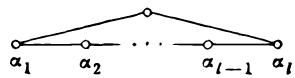
\includegraphics[keepaspectratio]{images/part002_112fabda.jpg}}

For \(l = 1\) , the Coxeter graph of the affine Weyl group is

\pandocbounded{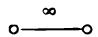
\includegraphics[keepaspectratio]{images/part002_c1e413d9.jpg}}

\begin{enumerate}
\def\labelenumi{(\Alph{enumi})}
\setcounter{enumi}{21}
\tightlist
\item
  \(R^{\prime} = R,\)
\end{enumerate}

\[
\Phi_ {\mathrm{R}} (x, y) = \frac {(x | y)}{2 (l + 1)}, \quad \gamma (\mathrm{R}) = (l + 1) ^ {2}.
\]

\begin{enumerate}
\def\labelenumi{(\Roman{enumi})}
\setcounter{enumi}{5}
\tightlist
\item
  Fundamental weights:
\end{enumerate}

\[
\begin{array}{l} \omega_ {i} = \varepsilon_ {1} + \dots + \varepsilon_ {i} - \frac {i}{l + 1} \sum_ {j = 1} ^ {l + 1} \varepsilon_ {j} \\ = \frac {1}{l + 1} [ (l - i + 1) (\alpha_ {1} + 2 \alpha_ {2} + \dots + (i - 1) \alpha_ {i - 1}) \\ \qquad + i ((l - i + 1) \alpha_ {i} + (l - i) \alpha_ {i + 1} + \dots + \alpha_ {l}) ]. \end{array}
\]

\begin{enumerate}
\def\labelenumi{(\Roman{enumi})}
\setcounter{enumi}{6}
\tightlist
\item
  Sum of the positive roots:
\end{enumerate}

\[
\begin{array}{c} 2 \rho = l \varepsilon_ {1} + (l - 2) \varepsilon_ {2} + (l - 4) \varepsilon_ {3} + \dots - (l - 2) \varepsilon_ {l} - l \varepsilon_ {l + 1} \\ = l \alpha_ {1} + 2 (l - 1) \alpha_ {2} + \dots + i (l - i + 1) \alpha_ {i} + \dots + l \alpha_ {l}. \end{array}
\]

\begin{enumerate}
\def\labelenumi{(\Roman{enumi})}
\setcounter{enumi}{7}
\item
  Q(R): the set of vectors whose coordinates are integers with sum zero. P(R): generated by Q(R) and \(\varepsilon_{1} - (l + 1)^{-1}(\varepsilon_{1} + \varepsilon_{2} + \cdots + \varepsilon_{l+1})\) . P(R)/Q(R) is isomorphic to Z/(l+1)Z. Connection index: l + 1.
\item
  Exponents: 1, 2, \ldots, l.
\item
  \(\mathrm{W}(\mathrm{R}) = \mathfrak{S}_{l + 1}\) , identified with the group of permutations of the \(\varepsilon_{i}\) . Order of \(\mathrm{W}(\mathrm{R})\colon (l + 1)!\)
\item
  \(l = 1\) : A(R) = W(R); \(w_0 = -1\) .
\end{enumerate}

\(l \geqslant 2: A(R) = W(R) \times \{1, -1\} \text{ and } w_{0} \text{ transforms } \alpha_{i} \text{ to } -\alpha_{l+1-i}.\)

\begin{enumerate}
\def\labelenumi{(\Roman{enumi})}
\setcounter{enumi}{11}
\item
  The group \(\mathrm{P}(\mathrm{R}^{-})/\mathrm{Q}(\mathrm{R}^{-})\) is cyclic of order \((l+1)\) ; it acts on the completed Dynkin graph by circular permutations. If \(l \geqslant 2\) , the unique non-identity element of \(\mathrm{A}(\mathrm{R})/\mathrm{W}(\mathrm{R})\) acts on \(\mathrm{P}(\mathrm{R})/\mathrm{Q}(\mathrm{R})\) by the automorphism \(x \mapsto -x\) .
\item
  Cartan matrix \((l \times l)\) :
\end{enumerate}

\[
\left( \begin{array}{c c c c c c c} 2 & - 1 & 0 & 0 & \dots & 0 & 0 \\ - 1 & 2 & - 1 & 0 & \dots & 0 & 0 \\ 0 & - 1 & 2 & - 1 & \dots & 0 & 0 \\ 0 & 0 & - 1 & 2 & \dots & 0 & 0 \\ \vdots & \vdots & \vdots & \vdots & \ddots & \vdots & \vdots \\ 0 & 0 & 0 & 0 & \dots & - 1 & 2 \end{array} \right)
\]

\specialchapter{\texorpdfstring{PLATE II. SYSTEMS OF TYPE \(B_{l}\) (\(l \geqslant 2\))}{PLATE II. SYSTEMS OF TYPE B\_l (l >= 2)}}

\begin{enumerate}
\def\labelenumi{(\Roman{enumi})}
\item
  \(V = E = R^{l}\) . Roots: \(\pm\varepsilon_{i}, (1\leqslant i\leqslant l), \pm\varepsilon_{i}\pm\varepsilon_{j} (1\leqslant i<j\leqslant l).\) Number of roots: \(n = 2l^{2}\) .
\item
  Basis: \(\alpha_{1} = \varepsilon_{1} - \varepsilon_{2},\alpha_{2} = \varepsilon_{2} - \varepsilon_{3},\ldots ,\alpha_{l - 1} = \varepsilon_{l - 1} - \varepsilon_{l},\alpha_{l} = \varepsilon_{l}\) . Positive roots:
\end{enumerate}

\[
\varepsilon_ {i} = \sum_ {i \leqslant k \leqslant l} \alpha_ {k} (1 \leqslant i \leqslant l),
\]

\[
\varepsilon_ {i} - \varepsilon_ {j} = \sum_ {i \leqslant k <   j} \alpha_ {k} (1 \leqslant i <   j \leqslant l),
\]

\[
\varepsilon_ {i} + \varepsilon_ {j} = \sum_ {i \leqslant k <   j} \alpha_ {k} + 2 \sum_ {j \leqslant k \leqslant l} \alpha_ {k} (1 \leqslant i <   j \leqslant l),
\]

\begin{enumerate}
\def\labelenumi{(\Roman{enumi})}
\setcounter{enumi}{2}
\item
  Coxeter number: \(h = 2l\) .
\item
  Highest root:
\end{enumerate}

\[
\tilde {\alpha} = \varepsilon_ {1} + \varepsilon_ {2} = \alpha_ {1} + 2 \alpha_ {2} + 2 \alpha_ {3} + \dots + 2 \alpha_ {l}.
\]

We have \(\tilde{\alpha} = 2\omega_{2}\) if \(l = 2\) , \(\tilde{\alpha} = \omega_{2}\) if \(l \geqslant 3\) .

Completed Dynkin graph:

for \(l = 2\) :

\pandocbounded{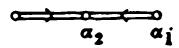
\includegraphics[keepaspectratio]{images/part002_ab2e3717.jpg}}

for \(l\geqslant 3\)

\pandocbounded{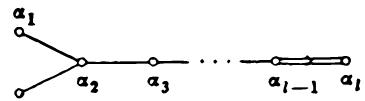
\includegraphics[keepaspectratio]{images/part002_677d35e2.jpg}}

\begin{enumerate}
\def\labelenumi{(\Alph{enumi})}
\setcounter{enumi}{21}
\tightlist
\item
  \(R^{\prime}\) is the set of vectors
\end{enumerate}

\[
\pm 2 \varepsilon_ {i} (1 \leqslant i \leqslant l), \pm \varepsilon_ {i} \pm \varepsilon_ {j} (1 \leqslant i <   j \leqslant l).
\]

\[
\Phi_ {\mathrm{R}} (x, y) = \frac {(x | y)}{4 l - 2}, \quad \gamma (\mathrm{R}) = (l + 1) (4 l - 2).
\]

\begin{enumerate}
\def\labelenumi{(\Roman{enumi})}
\setcounter{enumi}{5}
\tightlist
\item
  Fundamental weights:
\end{enumerate}

\[
\begin{array}{l} \omega_ {i} = \varepsilon_ {1} + \varepsilon_ {2} + \dots + \varepsilon_ {i} (1 \leqslant i <   l) \\ \quad = \alpha_ {1} + 2 \alpha_ {2} + \dots + (i - 1) \alpha_ {i - 1} + i (\alpha_ {i} + \alpha_ {i + 1} + \dots + \alpha_ {l}) \\ \omega_ {l} = \frac {1}{2} (\varepsilon_ {1} + \varepsilon_ {2} + \dots + \varepsilon_ {l}) \\ \quad = \frac {1}{2} (\alpha_ {1} + 2 \alpha_ {2} + \dots + l \alpha_ {l}). \end{array}
\]

\begin{enumerate}
\def\labelenumi{(\Roman{enumi})}
\setcounter{enumi}{6}
\tightlist
\item
  Sum of the positive roots:
\end{enumerate}

\[
\begin{array}{l} 2 \rho = (2 l - 1) \varepsilon_ {1} + (2 l - 3) \varepsilon_ {2} + \dots + 3 \varepsilon_ {l - 1} + \varepsilon_ {l} \\ = (2 l - 1) \alpha_ {1} + 2 (2 l - 2) \alpha_ {2} + \dots + i (2 l - i) \alpha_ {i} + \dots + l ^ {2} \alpha_ {l}. \end{array}
\]

\begin{enumerate}
\def\labelenumi{(\Roman{enumi})}
\setcounter{enumi}{7}
\tightlist
\item
  \(\mathrm{Q}(\mathrm{R}) = \bigoplus_{i=1}^{l}\mathbf{Z}\varepsilon_i,\mathrm{P}(\mathrm{R}) = \bigoplus_{i=1}^{l}\mathbf{Z}\varepsilon_i + \mathbf{Z}(\frac{1}{2}\sum_{i=1}^{l}\varepsilon_i).\)
\end{enumerate}

\(P(R)/Q(R)\) is isomorphic to Z/2Z, generated by the image of \(\omega_{l}\) . Connection index: 2.

\begin{enumerate}
\def\labelenumi{(\Roman{enumi})}
\setcounter{enumi}{8}
\item
  Exponents: 1, 3, 5, \ldots, 2l - 1.
\item
  W(R) is the semi-direct product of the group \(S_{l}\) , acting by permutations of the \(\varepsilon_{i}\) , by the group \((\mathbf{Z}/2\mathbf{Z})^{l}\) , acting by \(\varepsilon_{i} \mapsto (\pm1)_{i}\varepsilon_{i}\) . Its order is \(2^{l}.l!\)
\item
  A(R) = W(R); \(w_{0} = -1\) .
\item
  The unique non-trivial element of \(P(R^{\prime})/Q(R^{\prime})\) defines the unique non-trivial automorphism of the completed Dynkin graph.
\item
  Cartan matrix \((l \times l)\) :
\end{enumerate}

\[
\left( \begin{array}{c c c c c c c} 2 & - 1 & 0 & 0 & \dots & 0 & 0 \\ - 1 & 2 & - 1 & 0 & \dots & 0 & 0 \\ 0 & - 1 & 2 & - 1 & \dots & 0 & 0 \\ 0 & 0 & - 1 & 2 & \dots & 0 & 0 \\ \vdots & \vdots & \vdots & \vdots & \ddots & \vdots & \vdots \\ 0 & 0 & 0 & 0 & \dots & 2 & - 2 \\ 0 & 0 & 0 & 0 & \dots & - 1 & 2 \end{array} \right)
\]

\specialchapter{\texorpdfstring{PLATE III. SYSTEMS OF TYPE \(C_l\) (\(l \geqslant 2\))}{PLATE III. SYSTEMS OF TYPE C\_l (l >= 2)}}

\begin{enumerate}
\def\labelenumi{(\Roman{enumi})}
\item
  \(V = E = R^{l}.\) Roots: \(\pm2\varepsilon_{i}\) . ( \(1\leqslant i\leqslant l\) ). \(\pm\varepsilon_{i}\pm\varepsilon_{j}\) ( \(1\leqslant i<j\leqslant l\) ). Number of roots: \(n = 2l^{2}\) .
\item
  Basis: \(\alpha_{1} = \varepsilon_{1} - \varepsilon_{2},\alpha_{2} = \varepsilon_{2} - \varepsilon_{3},\ldots ,\alpha_{l - 1} = \varepsilon_{l - 1} - \varepsilon_{l},\alpha_{l} = 2\varepsilon_{l}\) Positive roots:
\end{enumerate}

\[
\varepsilon_ {i} - \varepsilon_ {j} = \sum_ {i \leqslant k <   j} \alpha_ {k} (1 \leqslant i <   j \leqslant l),
\]

\[
\varepsilon_ {i} + \varepsilon_ {j} = \sum_ {i \leqslant k <   j} \alpha_ {k} + 2 \sum_ {j \leqslant k <   l} \alpha_ {k} + \alpha_ {l} (1 \leqslant i <   j \leqslant l),
\]

\[
2 \varepsilon_ {i} = \sum_ {i \leqslant k <   l} \alpha_ {k} + \alpha_ {l} (1 \leqslant i \leqslant l).
\]

\begin{enumerate}
\def\labelenumi{(\Roman{enumi})}
\setcounter{enumi}{2}
\item
  Coxeter number: \(h = 2l\) .
\item
  Highest root:
\end{enumerate}

\[
\tilde {\alpha} = 2 \varepsilon_ {1} = 2 \alpha_ {1} + 2 \alpha_ {2} + \dots + 2 \alpha_ {l - 1} + \alpha_ {l}.
\]

Completed Dynkin graph:

\[
\alpha_ {1} \quad \alpha_ {2} \quad \dots \quad \alpha_ {l - 2} \quad \alpha_ {l - 1} \quad \alpha_ {l}
\]

\begin{enumerate}
\def\labelenumi{(\Alph{enumi})}
\setcounter{enumi}{21}
\tightlist
\item
  \(R^{\prime}\) is the set of vectors \(\pm\varepsilon_{i}\) . \(\pm\varepsilon_{i}\pm\varepsilon_{j}\) .
\end{enumerate}

\[
\Phi_ {\mathrm{R}} (x, y) = \frac {(x | y)}{4 (l + 1)}, \quad \gamma (\mathrm{R}) = (l + 1) (4 l - 2).
\]

\begin{enumerate}
\def\labelenumi{(\Roman{enumi})}
\setcounter{enumi}{5}
\tightlist
\item
  Fundamental weights:
\end{enumerate}

\[
\begin{array}{r l} \omega_ {i} & = \varepsilon_ {1} + \varepsilon_ {2} + \dots + \varepsilon_ {i} (1 \leqslant i \leqslant l) \\ & = \alpha_ {1} + 2 \alpha_ {2} + \dots + (i - 1) \alpha_ {i - 1} \\ & \quad + i (\alpha_ {i} + \alpha_ {i + 1} + \dots + \alpha_ {l - 1} + \frac {1}{2} \alpha_ {l}). \end{array}
\]

\begin{enumerate}
\def\labelenumi{(\Roman{enumi})}
\setcounter{enumi}{6}
\tightlist
\item
  Sum of the positive roots:
\end{enumerate}

\[
\begin{array}{r l} 2 \rho & = 2 l \varepsilon_ {1} + (2 l - 2) \varepsilon_ {2} + \dots + 4 \varepsilon_ {l - 1} + 2 \varepsilon_ {l} \\ & = 2 l \alpha_ {1} + 2 (2 l - 1) \alpha_ {2} + \dots + i (2 l - i + 1) \alpha_ {i} + \dots \\ & \qquad \dots + (l - 1) (l + 2) \alpha_ {l - 1} + \frac {1}{2} l (l + 1) \alpha_ {l}. \end{array}
\]

\begin{enumerate}
\def\labelenumi{(\Roman{enumi})}
\setcounter{enumi}{7}
\item
  Q(R): the set of points whose coordinates are integers with even sum. \(P(R) = \bigoplus_{i=1}^{l} Z \varepsilon_i\) . \(P(R)/Q(R)\) is isomorphic to \(Z/2Z\) , generated by the image of \(\omega_1\) .\\
  Connection index: 2.
\item
  Exponents: 1, 3, 5, \ldots, 2l - 1.
\item
  W(R) is the semi-direct product of the group \(S_{l}\) , acting by permutations of the \(\varepsilon_{i}\) , by the group \((\mathbf{Z}/2\mathbf{Z})^{l}\) , acting by \(\varepsilon_{i} \mapsto (\pm1)_{i}\varepsilon_{i}\) . Its order is \(2^{l}.l!\)
\item
  A(R) = W(R); \(w_{0} = -1\) .
\item
  The unique non-trivial element of \(P(R^{-})/Q(R^{-})\) defines the unique non-trivial automorphism of the completed Dynkin graph.
\item
  Cartan matrix \((l\times l)\) :
\end{enumerate}

\[
\left( \begin{array}{c c c c c c c} 2 & - 1 & 0 & 0 & \dots & 0 & 0 \\ - 1 & 2 & - 1 & 0 & \dots & 0 & 0 \\ 0 & - 1 & 2 & - 1 & \dots & 0 & 0 \\ 0 & 0 & - 1 & 2 & \dots & 0 & 0 \\ \vdots & \vdots & \vdots & \vdots & \ddots & \vdots & \vdots \\ 0 & 0 & 0 & 0 & \dots & 2 & - 1 \\ 0 & 0 & 0 & 0 & \dots & - 2 & 2 \end{array} \right)
\]

\specialchapter{\texorpdfstring{PLATE IV. SYSTEMS OF TYPE \(D_{l}\) (\(l \geqslant 3\))}{PLATE IV. SYSTEMS OF TYPE D\_l (l >= 3)}}

\begin{enumerate}
\def\labelenumi{(\Roman{enumi})}
\tightlist
\item
  \(V = E = R^{l}\) . Roots: \(\pm\varepsilon_{i}\pm\varepsilon_{j}(1\leqslant i<j\leqslant l)\) ; ( \(\varepsilon_{i}\) ) the canonical basis of \(R^{l}\) . Number of roots: \(n = 2l(l - 1)\) .
\end{enumerate}

\begin{enumerate}
\def\labelenumi{(\Roman{enumi})}
\setcounter{enumi}{1}
\tightlist
\item
  Basis: \(\alpha_{1} = \varepsilon_{1} - \varepsilon_{2},\alpha_{2} = \varepsilon_{2} - \varepsilon_{3},\ldots ,\alpha_{l - 1} = \varepsilon_{l - 1} - \varepsilon_{l},\alpha_{l} = \varepsilon_{l - 1} + \varepsilon_{l}\) . Positive roots:
\end{enumerate}

\[
\varepsilon_ {i} - \varepsilon_ {j} = \sum_ {i <   k <   j} \alpha_ {k} (1 \leqslant i <   j \leqslant l).
\]

\[
\varepsilon_ {i} + \varepsilon_ {l} = \sum_ {i \leqslant k \leqslant l - 2} \alpha_ {k} + \alpha_ {l} (1 \leqslant i <   l),
\]

\[
\varepsilon_ {i} + \varepsilon_ {j} = \sum_ {i \leqslant k <   j} \alpha_ {k} + 2 \sum_ {j \leqslant k <   l - 1} \alpha_ {k} + \alpha_ {l - 1} + \alpha_ {l} (1 \leqslant i <   j <   l).
\]

\begin{enumerate}
\def\labelenumi{(\Roman{enumi})}
\setcounter{enumi}{2}
\item
  Coxeter number: \(h = 2l - 2\) .
\item
  Highest root:
\end{enumerate}

\[
\tilde {\alpha} = \varepsilon_ {1} + \varepsilon_ {2} = \alpha_ {1} + 2 \alpha_ {2} + \dots + 2 \alpha_ {l - 2} + \alpha_ {l - 1} + \alpha_ {l}.
\]

We have \(\tilde{\alpha} = \omega_2 + \omega_3\) if \(l = 3\) and \(\tilde{\alpha} = \omega_2\) if \(l \geqslant 4\) .

Completed Dynkin graph (l ≥ 4):

\pandocbounded{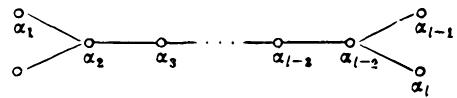
\includegraphics[keepaspectratio]{images/part002_b62b20f1.jpg}}

\begin{enumerate}
\def\labelenumi{(\Alph{enumi})}
\setcounter{enumi}{21}
\tightlist
\item
  \(R^{\prime} = R.\)
\end{enumerate}

\[
\Phi_ {R} (x, y) = \frac {(x | y)}{4 (l - 1)}, \quad \gamma (R) = 4 (l - 1) ^ {2}.
\]

\begin{enumerate}
\def\labelenumi{(\Roman{enumi})}
\setcounter{enumi}{5}
\tightlist
\item
  Fundamental weights:
\end{enumerate}

\[
\begin{array}{r l} \omega_ {i} & = \varepsilon_ {1} + \varepsilon_ {2} + \dots + \varepsilon_ {i} (1 \leqslant i \leqslant l - 2) \\ & = \alpha_ {1} + 2 \alpha_ {2} + \dots + (i - 1) \alpha_ {i - 1} + i (\alpha_ {i} + \alpha_ {i + 1} + \dots + \alpha_ {l - 2}) \\ & \quad + \frac {1}{2} i (\alpha_ {l - 1} + \alpha_ {l}) \\ \omega_ {l - 1} & = \frac {1}{2} (\varepsilon_ {1} + \varepsilon_ {2} + \dots + \varepsilon_ {l - 2} + \varepsilon_ {l - 1} - \varepsilon_ {l}) \\ & = \frac {1}{2} (\alpha_ {1} + 2 \alpha_ {2} + \dots + (l - 2) \alpha_ {l - 2} + \frac {1}{2} l \alpha_ {l - 1} + \frac {1}{2} (l - 2) \alpha_ {l}) \\ \omega_ {l} & = \frac {1}{2} (\varepsilon_ {1} + \varepsilon_ {2} + \dots + \varepsilon_ {l - 2} + \varepsilon_ {l - 1} + \varepsilon_ {l}) \\ & = \frac {1}{2} (\alpha_ {1} + 2 \alpha_ {2} + \dots + (l - 2) \alpha_ {l - 2} + \frac {1}{2} (l - 2) \alpha_ {l - 1} + \frac {1}{2} l \alpha_ {l}). \end{array}
\]

\begin{enumerate}
\def\labelenumi{(\Roman{enumi})}
\setcounter{enumi}{6}
\tightlist
\item
  Sum of the positive roots:
\end{enumerate}

\[
\begin{array}{r l} 2 \rho & = 2 (l - 1) \varepsilon_ {1} + 2 (l - 2) \varepsilon_ {2} + \dots + 2 \varepsilon_ {l - 1} \\ & = 2 (l - 1) \alpha_ {1} + 2 (2 l - 3) \alpha_ {2} + \dots + 2 (i l - \frac {i (i + 1)}{2}) \alpha_ {i} + \dots \\ & \qquad \dots + \frac {l (l - 1)}{2} (\alpha_ {l - 1} + \alpha_ {l}). \end{array}
\]

\begin{enumerate}
\def\labelenumi{(\Roman{enumi})}
\setcounter{enumi}{7}
\tightlist
\item
  Q(R): the set of points whose coordinates are integers with even sum.
\end{enumerate}

\[
\mathrm{P} (\mathrm{R}) = \bigoplus_ {i = 1} ^ {l} \mathbf {Z} \varepsilon_ {i} + \mathbf {Z} \left(\frac {1}{2} \sum_ {i = 1} ^ {l} \varepsilon_ {i}\right).
\]

l odd: \(\mathrm{P}(\mathrm{R})/\mathrm{Q}(\mathrm{R})\) is isomorphic to Z/4Z, generated by the image of \(\omega_{l}\) ; we have \(\omega_{1} \equiv 2\omega_{l}\) and \(\omega_{l-1} \equiv 3\omega_{l} \mod Q(\mathrm{R})\) . l even: \(\mathrm{P}(\mathrm{R})/\mathrm{Q}(\mathrm{R})\) is isomorphic to \((\mathbf{Z}/2\mathbf{Z}) \times (\mathbf{Z}/2\mathbf{Z})\) ; the three elements of order 2 are the images of \(\omega_{1}, \omega_{l-1}\) and \(\omega_{l}\) . Connection index: 4.

\begin{enumerate}
\def\labelenumi{(\Roman{enumi})}
\setcounter{enumi}{8}
\item
  Exponents: 1, 3, 5, \ldots, 2l - 5, 2l - 3, l - 1 (the last appearing twice if l is even and once if l is odd).
\item
  W(R) is the semi-direct product of the group \(S_{l}\) , acting by permutations of the \(\varepsilon_{i}\) , by the group \((\mathbf{Z}/2\mathbf{Z})^{l-1}\) , acting by \(\varepsilon_{i} \mapsto (\pm1)_{i}\varepsilon_{i}\) with \(\prod_{i}(\pm1)_{i} = 1\) . Its order is \(2^{l-1}.l!\)
\item
  \(l \neq 4\) : A(R)/W(R) = Z/2Z acting on the Dynkin graph by transposition of the nodes \(\alpha_{l-1}\) and \(\alpha_l\) . \(l = 4\) : A(R)/W(R) = \(\mathfrak{S}_3\) , acting on the Dynkin graph by permuting the nodes \(\alpha_1, \alpha_3\) and \(\alpha_4\) . \(w_0 = -1\) if \(l\) is even; \(w_0 = -\varepsilon\) if \(l\) is odd. where \(\varepsilon\) is the automorphism that interchanges \(\alpha_{l-1}\) and \(\alpha_l\) and leaves the other \(\alpha_i\) fixed.
\item
  Action of \(\mathrm{P}(\mathbb{R}^{-}) / \mathrm{Q}(\mathbb{R}^{-}) = \mathrm{P}(\mathbb{R}) / \mathrm{Q}(\mathbb{R})\) on the completed Dynkin graph: \(l\) odd: \(\omega_l\) transforms \(\alpha_0\) into \(\alpha_1\) , \(\alpha_l\) into \(\alpha_1\) , \(\alpha_1\) into \(\alpha_{l-1}\) and \(\alpha_{l-1}\) into \(\alpha_0\) ; it interchanges \(\alpha_j\) and \(\alpha_{l-j}\) for \(2 \leqslant j \leqslant l - 2\) . \(l\) even: \(\omega_l\) (resp. \(\omega_{l-1}\) ) interchanges \(\alpha_0\) and \(\alpha_l\) (resp. \(\alpha_0\) and \(\alpha_{l-1}\) ), \(\alpha_1\) and \(\alpha_{l-1}\) (resp. \(\alpha_1\) and \(\alpha_l\) ) and interchanges \(\alpha_j\) and \(\alpha_{l-j}\) for \(2 \leqslant j \leqslant l - 2\) .
\end{enumerate}

\[
\left( \begin{array}{c c c c c c c} 2 & - 1 & \dots & 0 & 0 & 0 & 0 \\ - 1 & 2 & \dots & 0 & 0 & 0 & 0 \\ \vdots & \vdots & \ddots & \vdots & \vdots & \vdots & \vdots \\ 0 & 0 & \dots & 2 & - 1 & 0 & 0 \\ 0 & 0 & \dots & - 1 & 2 & - 1 & - 1 \\ 0 & 0 & \dots & 0 & - 1 & 2 & 0 \\ 0 & 0 & \dots & 0 & - 1 & 0 & 2 \end{array} \right)
\]

\begin{enumerate}
\def\labelenumi{(\Roman{enumi})}
\setcounter{enumi}{12}
\tightlist
\item
  Cartan matrix \((l\times l)\) :
\end{enumerate}

\specialchapter{\texorpdfstring{PLATE V. SYSTEM OF TYPE \(E_{6}\)}{PLATE V. SYSTEM OF TYPE E\_6}}

\begin{enumerate}
\def\labelenumi{(\Roman{enumi})}
\tightlist
\item
  V is the subspace of \(E = R^{8}\) consisting of the points whose coordinates \((\xi_{i})\) are such that \(\xi_{6} = \xi_{7} = -\xi_{8}\) . Roots: \(\pm\varepsilon_{i} \pm \varepsilon_{j} (1 \leqslant i < j \leqslant 5)\) ,
\end{enumerate}

\[
\pm \frac {1}{2} (\varepsilon_ {8} - \varepsilon_ {7} - \varepsilon_ {6} + \sum_ {i = 1} ^ {5} (- 1) ^ {\nu (i)} \varepsilon_ {i}) \text {with} \sum_ {i = 1} ^ {5} \nu (i) \text {even.}
\]

Number of roots: n = 72.

\begin{enumerate}
\def\labelenumi{(\Roman{enumi})}
\setcounter{enumi}{1}
\tightlist
\item
Basis: \(\alpha_{1} = \frac{1}{2} (\varepsilon_{1} + \varepsilon_{8}) - \frac{1}{2} (\varepsilon_{2} + \varepsilon_{3} + \varepsilon_{4} + \varepsilon_{5} + \varepsilon_{6} + \varepsilon_{7}),\alpha_{2} = \varepsilon_{1} + \varepsilon_{2},\alpha_{3} =\) \(\varepsilon_2 - \varepsilon_1,\alpha_4 = \varepsilon_3 - \varepsilon_2,\alpha_5 = \varepsilon_4 - \varepsilon_3,\alpha_6 = \varepsilon_5 - \varepsilon_4.\) Positive roots: \(\pm \varepsilon_i + \varepsilon_j\) \(1\leqslant i <   j\leqslant 5)\)
\end{enumerate}

\[
\frac {1}{2} \left(\varepsilon_ {8} - \varepsilon_ {7} - \varepsilon_ {6} + \sum_ {i = 1} ^ {5} (- 1) ^ {\nu (i)} \varepsilon_ {i}\right) \text {with} \sum_ {i = 1} ^ {5} \nu (i) \text {even}.
\]

Positive roots with at least one coefficient \(\geqslant 2\) (we denote the root \(a\alpha_{1} + b\alpha_{2} + c\alpha_{3} + d\alpha_{4} + e\alpha_{5} + f\alpha_{6}\) ) by \({ }^{a c d e f}_{b})^{13}\) :

\[
\begin{array}{c c c c c c} 0   1   2   1   0 & 1   1   2   1   0 & 0   1   2   1   1 & 1   2   2   1   0 & 1   1   2   1   1 & 0   1   2   2   1 \\ 1 & 1 & 1 & 1 & 1 & 1 \\ 1   2   2   1   1 & 1   1   2   2   1 & 1   2   2   2   1 & 1   2   3   2   1 & 1   2   3   2   1 \\ 1 & 1 & 1 & 1 & 2 \end{array}
\]

\begin{enumerate}
\def\labelenumi{(\Roman{enumi})}
\setcounter{enumi}{2}
\item
  Coxeter number: \(h = 12\) .
\item
  Highest root:
\end{enumerate}

\[
\begin{array}{r l} \tilde {\alpha} & = \frac {1}{2} (\varepsilon_ {1} + \varepsilon_ {2} + \varepsilon_ {3} + \varepsilon_ {4} + \varepsilon_ {5} - \varepsilon_ {6} - \varepsilon_ {7} + \varepsilon_ {8}) \\ & = \alpha_ {1} + 2 \alpha_ {2} + 2 \alpha_ {3} + 3 \alpha_ {4} + 2 \alpha_ {5} + \alpha_ {6} = \omega_ {2}. \end{array}
\]

Completed Dynkin graph:

\pandocbounded{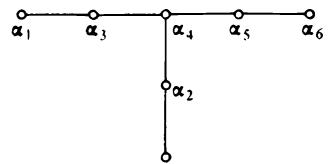
\includegraphics[keepaspectratio]{images/part002_985a73c0.jpg}}

\begin{enumerate}
\def\labelenumi{(\Alph{enumi})}
\setcounter{enumi}{21}
\tightlist
\item
  \(R^{\prime} = R.\)
\end{enumerate}

\[
  \Phi_ {\mathrm{R}} (x, y) = (x | y) / 24, \quad \gamma (\mathrm{R}) = 144.
\]

\begin{enumerate}
\def\labelenumi{(\Roman{enumi})}
\setcounter{enumi}{5}
\tightlist
\item
  Fundamental weights:
\end{enumerate}

\[
\begin{array}{l} \omega_ {1} = \frac {2}{3} (\varepsilon_ {8} - \varepsilon_ {7} - \varepsilon_ {6}) = \frac {1}{3} (4 \alpha_ {1} + 3 \alpha_ {2} + 5 \alpha_ {3} + 6 \alpha_ {4} + 4 \alpha_ {5} + 2 \alpha_ {6}) \\ \omega_ {2} = \frac {1}{2} (\varepsilon_ {1} + \varepsilon_ {2} + \varepsilon_ {3} + \varepsilon_ {4} + \varepsilon_ {5} - \varepsilon_ {6} - \varepsilon_ {7} + \varepsilon_ {8}) \\ \quad = \alpha_ {1} + 2 \alpha_ {2} + 2 \alpha_ {3} + 3 \alpha_ {4} + 2 \alpha_ {5} + \alpha_ {6} = \tilde {\alpha} \\ \omega_ {3} = \frac {5}{6} (\varepsilon_ {8} - \varepsilon_ {7} - \varepsilon_ {6}) + \frac {1}{2} (- \varepsilon_ {1} + \varepsilon_ {2} + \varepsilon_ {3} + \varepsilon_ {4} + \varepsilon_ {5}) \\ \quad = \frac {1}{3} (5 \alpha_ {1} + 6 \alpha_ {2} + 10 \alpha_ {3} + 12 \alpha_ {4} + 8 \alpha_ {5} + 4 \alpha_ {6}) \\ \omega_ {4} = \varepsilon_ {3} + \varepsilon_ {4} + \varepsilon_ {5} - \varepsilon_ {6} - \varepsilon_ {7} + \varepsilon_ {8} \\ \quad = 2 \alpha_ {1} + 3 \alpha_ {2} + 4 \alpha_ {3} + 6 \alpha_ {4} + 4 \alpha_ {5} + 2 \alpha_ {6} \\ \omega_ {5} = \frac {2}{3} (\varepsilon_ {8} - \varepsilon_ {7} - \varepsilon_ {6}) + \varepsilon_ {4} + \varepsilon_ {5} \\ \quad = \frac {1}{3} (4 \alpha_ {1} + 6 \alpha_ {2} + 8 \alpha_ {3} + 12 \alpha_ {4} + 10 \alpha_ {5} + 5 \alpha_ {6}) \\ \omega_ {6} = \frac {1}{3} (\varepsilon_ {8} - \varepsilon_ {7} - \varepsilon_ {6}) + \varepsilon_ {5} \\ \quad = \frac {1}{3} (2 \alpha_ {1} + 3 \alpha_ {2} + 4 \alpha_ {3} + 6 \alpha_ {4} + 5 \alpha_ {5} + 4 \alpha_ {6}). \end{array}
\]

\begin{enumerate}
\def\labelenumi{(\Roman{enumi})}
\setcounter{enumi}{6}
\tightlist
\item
  Sum of the positive roots:
\end{enumerate}

\[
\begin{array}{l} 2 \rho = 2 (\varepsilon_ {2} + 2 \varepsilon_ {3} + 3 \varepsilon_ {4} + 4 \varepsilon_ {5} + 4 (\varepsilon_ {8} - \varepsilon_ {7} - \varepsilon_ {6})) \\ = 2 (8 \alpha_ {1} + 11 \alpha_ {2}) + 15 \alpha_ {3} + 21 \alpha_ {4} + 15 \alpha_ {5} + 8 \alpha_ {6}). \end{array}
\]

\begin{enumerate}
\def\labelenumi{(\Roman{enumi})}
\setcounter{enumi}{7}
\tightlist
\item
  P(R)/Q(R) is isomorphic to Z/3Z.
\end{enumerate}

Connection index: 3.

\begin{enumerate}
\def\labelenumi{(\Roman{enumi})}
\setcounter{enumi}{8}
\item
  Exponents: 1, 4, 5, 7, 8, 11.
\item
  Order of W(R): \(2^{7}.3^{4}.5\) .
\item
  \(\mathrm{A}(\mathrm{R}) = \mathrm{W}(\mathrm{R}) \times \{1, -1\}\) ; \(w_0\) transforms \(\alpha_1, \alpha_2, \alpha_3, \alpha_4, \alpha_5, \alpha_6\) , respectively, into \(-\alpha_6, -\alpha_2, -\alpha_5, -\alpha_4, -\alpha_3, -\alpha_1\) .
\item
  The non-identity element of \(\mathrm{A}(\mathbb{R}) / \mathrm{W}(\mathbb{R})\) defines the automorphism \(x \mapsto -x\) of \(\mathrm{P}(\mathbb{R}) / \mathrm{Q}(\mathbb{R})\) .
\end{enumerate}

The group of automorphisms of the completed Dynkin diagram is isomorphic to \(S_{3}\) ; its elements of order 3 are induced by the two non-trivial elements of \(P(R^{-})/Q(R^{-})\) .

\[
\left( \begin{array}{c c c c c c} 2 & 0 & - 1 & 0 & 0 & 0 \\ 0 & 2 & 0 & - 1 & 0 & 0 \\ - 1 & 0 & 2 & - 1 & 0 & 0 \\ 0 & - 1 & - 1 & 2 & - 1 & 0 \\ 0 & 0 & 0 & - 1 & 2 & - 1 \\ 0 & 0 & 0 & 0 & - 1 & 2 \end{array} \right)
\]

\begin{enumerate}
\def\labelenumi{(\Roman{enumi})}
\setcounter{enumi}{12}
\tightlist
\item
  Cartan matrix:
\end{enumerate}

\specialchapter{\texorpdfstring{PLATE VI. SYSTEM OF TYPE \(E_{7}\)}{PLATE VI. SYSTEM OF TYPE E\_7}}

\begin{enumerate}
\def\labelenumi{(\Roman{enumi})}
\tightlist
\item
  V is the hyperplane in \(E = R^{8}\) orthogonal to \(\varepsilon_{7} + \varepsilon_{8}\) .
\end{enumerate}

Roots: \(\pm \varepsilon_{i} \pm \varepsilon_{j} (1 \leqslant i < j \leqslant 6)\) , \(\pm (\varepsilon_{7} - \varepsilon_{8})\) ,

\[
\pm \frac {1}{2} (\varepsilon_ {7} - \varepsilon_ {8} + \sum_ {i = 1} ^ {6} (- 1) ^ {\nu (i)} \varepsilon_ {i}) \quad \text { with } \sum_ {i = 1} ^ {8} \nu (i) \text { odd. }
\]

Number of roots: n = 126.

\begin{enumerate}
\def\labelenumi{(\Roman{enumi})}
\setcounter{enumi}{1}
\tightlist
\item
  Basis:
\end{enumerate}

\[
\begin{array}{r l} \alpha_ {1} & = \frac {1}{2} (\varepsilon_ {1} + \varepsilon_ {8}) - \frac {1}{2} (\varepsilon_ {2} + \varepsilon_ {3} + \varepsilon_ {4} + \varepsilon_ {5} + \varepsilon_ {6} + \varepsilon_ {7}), \\ \alpha_ {2} & = \varepsilon_ {1} + \varepsilon_ {2}, \alpha_ {3} = \varepsilon_ {2} - \varepsilon_ {1}, \alpha_ {4} = \varepsilon_ {3} - \varepsilon_ {2}, \alpha_ {5} = \varepsilon_ {4} - \varepsilon_ {3}, \\ \alpha_ {6} & = \varepsilon_ {5} - \varepsilon_ {4}, \alpha_ {7} = \varepsilon_ {6} - \varepsilon_ {5}. \end{array}
\]

Positive roots:

\[
\begin{array}{c} \pm \varepsilon_ {i} + \varepsilon_ {j} (1 \leqslant i <   j \leqslant 6), - \varepsilon_ {7} + \varepsilon_ {8}, \\ \frac {1}{2} (- \varepsilon_ {7} + \varepsilon_ {8} + \sum_ {i = 1} ^ {6} (- 1) ^ {\nu (i)} \varepsilon_ {i}) \quad \text { with } \sum_ {i = 1} ^ {6} \nu (i) \text { odd }. \end{array}
\]

Positive roots containing \(\alpha_{7}\) and having at least one coefficient \(\geqslant 2\) (we denote the root \(a\alpha_{1} + b\alpha_{2} + c\alpha_{3} + d\alpha_{4} + e\alpha_{5} + f\alpha_{6} + g\alpha_{7}\) by \(\frac{a c d e f g}{b})^{14}\) :

\[
\begin{array}{c c c c c} 0   1   2   1   1   1 & 1   1   2   1   1   1 & 0   1   2   2   1   1 & 1   2   2   1   1   1 & 1   1   2   2   1   1 \\ 1 & 1 & 1 & 1 & 1 \\ 0   1   2   2   2   1 & 1   2   2   2   1   1 & 1   1   2   2   2   1 & 1   2   2   2   2   1 & 1   2   3   2   1   1 \\ 1 & 1 & 1 & 1 & 1 \\ 1   2   3   2   2   1 & 1   2   3   2   1   1 & 1   2   3   3   2   1 & 1   2   3   2   2   1 & 1   2   3   3   2   1 \\ 1 & 2 & 1 & 2 & 2 \end{array}
\]

\[
\begin{array}{c c c} 1 2 4 3 2 1 & 1 3 4 3 2 1 & 2 3 4 3 2 1 \\ 2 & 2 & 2 \end{array}
\]

\begin{enumerate}
\def\labelenumi{(\Roman{enumi})}
\setcounter{enumi}{2}
\item
  Coxeter number: \(h = 18\) .
\item
  Highest root:
\end{enumerate}

\[
\tilde {\alpha} = \varepsilon_ {8} - \varepsilon_ {7} = 2 \alpha_ {1} + 2 \alpha_ {2} + 3 \alpha_ {3} + 4 \alpha_ {4} + 3 \alpha_ {5} + 2 \alpha_ {6} + \alpha_ {7} = \omega_ {1}.
\]

Completed Dynkin graph:

\[
\alpha_ {1} \quad \alpha_ {3} \quad \alpha_ {4} \quad \alpha_ {5} \quad \alpha_ {6} \quad \alpha_ {7}
\]

\begin{enumerate}
\def\labelenumi{(\Alph{enumi})}
\setcounter{enumi}{21}
\tightlist
\item
  \(R^{\prime} = R.\)
\end{enumerate}

\[
  \Phi_ {\mathrm{R}} (x, y) = (x | y) / 36, \quad \gamma (\mathrm{R}) = 2 ^ {2}. 3 ^ {4}.
\]

\begin{enumerate}
\def\labelenumi{(\Roman{enumi})}
\setcounter{enumi}{5}
\tightlist
\item
  Fundamental weights:
\end{enumerate}

\[
\begin{array}{l} \omega_ {1} = \varepsilon_ {8} - \varepsilon_ {7} = 2 \alpha_ {1} + 2 \alpha_ {2} + 3 \alpha_ {3} + 4 \alpha_ {4} + 3 \alpha_ {5} + 2 \alpha_ {6} + \alpha_ {7} \\ \omega_ {2} = \frac {1}{2} (\varepsilon_ {1} + \varepsilon_ {2} + \varepsilon_ {3} + \varepsilon_ {4} + \varepsilon_ {5} + \varepsilon_ {6} - 2 \varepsilon_ {7} + 2 \varepsilon_ {8}) \\ \qquad = \frac {1}{2} (4 \alpha_ {1} + 7 \alpha_ {2} + 8 \alpha_ {3} + 12 \alpha_ {4} + 9 \alpha_ {5} + 8 \alpha_ {6} + 3 \alpha_ {7}) \\ \omega_ {3} = \frac {1}{2} (- \varepsilon_ {1} + \varepsilon_ {2} + \varepsilon_ {3} + \varepsilon_ {4} + \varepsilon_ {5} + \varepsilon_ {6} - 3 \varepsilon_ {7} + 3 \varepsilon_ {8}) \\ \qquad = 3 \alpha_ {1} + 4 \alpha_ {2} + 6 \alpha_ {3} + 8 \alpha_ {4} + 6 \alpha_ {5} + 4 \alpha_ {6} + 2 \alpha_ {7} \\ \omega_ {4} = \varepsilon_ {3} + \varepsilon_ {4} + \varepsilon_ {5} + \varepsilon_ {6} + 2 (\varepsilon_ {8} - \varepsilon_ {7}) \\ \qquad = 4 \alpha_ {1} + 6 \alpha_ {2} + 8 \alpha_ {3} + 12 \alpha_ {4} + 9 \alpha_ {5} + 6 \alpha_ {6} + 3 \alpha_ {7} \\ \omega_ {5} = \varepsilon_ {4} + \varepsilon_ {5} + \varepsilon_ {6} + \frac {3}{2} (\varepsilon_ {8} - \varepsilon_ {7}) \\ \qquad = \frac {1}{2} (6 \alpha_ {1} + 9 \alpha_ {2} + 12 \alpha_ {3} + 18 \alpha_ {4} + 15 \alpha_ {5} + 10 \alpha_ {6} + 5 \alpha_ {7}) \\ \omega_ {6} = \varepsilon_ {5} + \varepsilon_ {6} - \varepsilon_ {7} + \varepsilon_ {8} \\ \qquad = 2 \alpha_ {1} + 3 \alpha_ {2} + 4 \alpha_ {3} + 6 \alpha_ {4} + 5 \alpha_ {5} + 4 \alpha_ {6} + 2 \alpha_ {7} \\ \omega_ {7} = \varepsilon_ {6} + \frac {1}{2} (\varepsilon_ {8} - \varepsilon_ {7}) \\ \qquad = \frac {1}{2} (2 \alpha_ {1} + 3 \alpha_ {2} + 4 \alpha_ {3} + 6 \alpha_ {4} + 5 \alpha_ {5} + 4 \alpha_ {6} + 3 \alpha_ {7}). \end{array}
\]

\begin{enumerate}
\def\labelenumi{(\Roman{enumi})}
\setcounter{enumi}{6}
\tightlist
\item
  Sum of the positive roots:
\end{enumerate}

\[
\begin{array}{l} 2 \rho = 2 \varepsilon_ {2} + 4 \varepsilon_ {3} + 6 \varepsilon_ {4} + 8 \varepsilon_ {5} + 10 \varepsilon_ {6} - 17 \varepsilon_ {7} + 17 \varepsilon_ {8} \\ = 34 \alpha_ {1} + 49 \alpha_ {2} + 66 \alpha_ {3} + 96 \alpha_ {4} + 75 \alpha_ {5} + 52 \alpha_ {6} + 27 \alpha_ {7}. \end{array}
\]


\begin{enumerate}
\def\labelenumi{(\Roman{enumi})}
\setcounter{enumi}{7}
\item
  P(R)/Q(R) is isomorphic to Z/2Z. Connection index: 2.
\item
  Exponents: 1, 5, 7, 9, 11, 13, 17.
\item
  Order of W(R): \(2^{10}.3^{4}.5.7\) .
\item
  A(R) = W(R), \(w_{0} = -1\) .
\item
  \(P(R^{\prime})/Q(R^{\prime})\) has only one non-identity element: it defines the unique non-trivial automorphism of the Dynkin graph.
\end{enumerate}

\[
\left( \begin{array}{c c c c c c c} 2 & 0 & - 1 & 0 & 0 & 0 & 0 \\ 0 & 2 & 0 & - 1 & 0 & 0 & 0 \\ - 1 & 0 & 2 & - 1 & 0 & 0 & 0 \\ 0 & - 1 & - 1 & 2 & - 1 & 0 & 0 \\ 0 & 0 & 0 & - 1 & 2 & - 1 & 0 \\ 0 & 0 & 0 & 0 & - 1 & 2 & - 1 \\ 0 & 0 & 0 & 0 & 0 & - 1 & 2 \end{array} \right)
\]

\begin{enumerate}
\def\labelenumi{(\Roman{enumi})}
\setcounter{enumi}{12}
\tightlist
\item
  Cartan matrix:
\end{enumerate}

\specialchapter{\texorpdfstring{PLATE VII. SYSTEM OF TYPE \(\mathbf{E}_8\)}{PLATE VII. SYSTEM OF TYPE E\_8}}

\begin{enumerate}
\def\labelenumi{(\Roman{enumi})}
\tightlist
\item
  \(V = E = R^{8}.\)
\end{enumerate}

\[
\begin{array}{l} \text {Roots:} \pm \varepsilon_ {i} \pm \varepsilon_ {j} (i <   j), \frac {1}{2} \sum_ {i = 1} ^ {8} (- 1) ^ {\nu (\mathrm{i})} \varepsilon_ {i} \text {with} \sum_ {i = 1} ^ {8} \nu (i) \text {even.} \\ \text {Number of roots:} n = 240. \end{array}
\]

\begin{enumerate}
\def\labelenumi{(\Roman{enumi})}
\setcounter{enumi}{1}
\tightlist
\item
  Basis:
\end{enumerate}

\[
\begin{array}{r l} \alpha_ {1} & = \frac {1}{2} (\varepsilon_ {1} + \varepsilon_ {8}) - \frac {1}{2} (\varepsilon_ {2} + \varepsilon_ {3} + \varepsilon_ {4} + \varepsilon_ {5} + \varepsilon_ {6} + \varepsilon_ {7}), \\ \alpha_ {2} & = \varepsilon_ {1} + \varepsilon_ {2}, \alpha_ {3} = \varepsilon_ {2} - \varepsilon_ {1}, \alpha_ {4} = \varepsilon_ {3} - \varepsilon_ {2}, \alpha_ {5} = \varepsilon_ {4} - \varepsilon_ {3}, \\ \alpha_ {6} & = \varepsilon_ {5} - \varepsilon_ {4}, \alpha_ {7} = \varepsilon_ {6} - \varepsilon_ {5}, \alpha_ {8} = \varepsilon_ {7} - \varepsilon_ {6}. \end{array}
\]

Positive roots:

\[
\pm \varepsilon_ {i} + \varepsilon_ {j} (i <   j), \frac {1}{2} (\varepsilon_ {8} + \sum_ {i = 1} ^ {7} (- 1) ^ {\nu (\mathrm{i})} \varepsilon_ {i}) \text {with} \sum_ {i = 1} ^ {7} \nu (i) \text {even}.
\]

Positive roots containing \(\alpha_{8}\) and having at least one coefficient \(\geqslant 2\) (we denote the root \(a\alpha_{1} + b\alpha_{2} + c\alpha_{3} + d\alpha_{4} + e\alpha_{5} + f\alpha_{6} + g\alpha_{7} + h\alpha_{8}\) by \(\left.\frac{a}{b}c\frac{d}{e}\frac{e}{f}\frac{g}{h}\right)^{15}\) :

\[
\begin{array}{c c c c c} 0   1   2   1   1   1   1 & 0   1   2   2   1   1   1 & 1   1   2   1   1   1   1 & 0   1   2   2   2   1   1 & 1   2   2   1   1   1   1 \\ 1 & 1 & 1 & 1 & 1 \\ 1   1   2   2   1   1   1 & 1   2   2   2   1   1   1 & 1   1   2   2   2   1   1 & 0   1   2   2   2   2   1 & 1   2   3   2   1   1   1 \\ 1 & 1 & 1 & 1 & 1 \\ 1   2   2   2   2   1   1 & 1   1   2   2   2   2   1 & 1   2   3   2   2   1   1 & 1   2   3   2   2   1   1 & 1   2   2   2   2   2   1 \\ 1 & 1 & 2 & 1 & 1 \\ 1   2   3   2   2   1   1 & 1   2   3   3   2   1   1 & 1   2   3   2   2   2   1 & 1   2   3   3   2   1   1 & 1   2   3   2   2   2   1 \\ 2 & 1 & 1 & 2 & 2 \end{array}
\]

\[
\begin{array}{c c c c c} 1   2   3   3   3   2   1 & 1   2   4   3   2   1   1 & 1   2   3   3   2   2   1 & 1   2   3   3   3   2   1 & 1   3   4   3   2   1   1 \\ 1 & 2 & 2 & 1 & 2 \\ 1   2   4   3   2   2   1 & 1   2   3   3   3   2   1 & 2   3   4   3   2   1   1 & 1   3   4   3   2   2   1 & 1   2   4   3   3   2   1 \\ 2 & 2 & 2 & 2 & 2 \\ 2   3   4   3   2   2   1 & 1   3   4   3   3   2   1 & 1   2   4   4   3   2   1 & 2   3   4   3   3   2   1 & 1   3   4   4   3   2   1 \\ 2 & 2 & 2 & 2 & 2 \\ 1   3   5   4   3   2   1 & 2   3   4   4   3   2   1 & 1   3   5   4   3   2   1 & 2   3   5   4   3   2   1 & 2   3   5   4   3   2   1 \\ 2 & 2 & 3 & 2 & 3 \\ \text { } _ {2} ^ {2} \text { } _ {5} ^ {4} \text { } _ {5} ^ {4} \text { } _ {5} ^ {4} \text { } _ {5} ^ {4} \text { } _ {5} ^ {4} \text { } _ {5} ^ {4} \text { } _ {5} ^ {4} \text { } _ {5} ^ {4} \text { } _ {5} ^ {4} \text {(} _ {2} ^ {2} \text {)} _ {2} ^ {3} \text {)} _ {3} ^ {3} \text {)} _ {3} ^ {3} \text {)} _ {3} ^ {3} \end{array}
\]

\begin{enumerate}
\def\labelenumi{(\Roman{enumi})}
\setcounter{enumi}{2}
\item
  Coxeter number: \(h = 30\) .
\item
  Highest root:
\end{enumerate}

\[
\begin{array}{r l} \tilde {\alpha} & = \varepsilon_ {7} + \varepsilon_ {8} = 2 \alpha_ {1} + 3 \alpha_ {2} + 4 \alpha_ {3} + 6 \alpha_ {4} + 5 \alpha_ {5} + 4 \alpha_ {6} + 3 \alpha_ {7} + 2 \alpha_ {8} \\ & = \omega_ {8}. \end{array}
\]

Completed Dynkin graph is:

\[
\begin{array}{c} \alpha_ {1} \quad \alpha_ {3} \\ \alpha_ {4} \quad \alpha_ {5} \quad \alpha_ {6} \quad \alpha_ {7} \quad \alpha_ {8} \\ \alpha_ {2} \end{array}
\]

\begin{enumerate}
\def\labelenumi{(\Alph{enumi})}
\setcounter{enumi}{21}
\tightlist
\item
  \(R^{\prime} = R.\)
\end{enumerate}

\[
  \Phi_ {\mathrm{R}} (x, y) = (x | y) / 60, \quad \gamma (\mathrm{R}) = 900.
\]

\begin{enumerate}
\def\labelenumi{(\Roman{enumi})}
\setcounter{enumi}{5}
\tightlist
\item
  Fundamental weights:
\end{enumerate}

\[
\begin{array}{l} \omega_ {1} = 2 \varepsilon_ {8} = 4 \alpha_ {1} + 5 \alpha_ {2} + 7 \alpha_ {3} + 10 \alpha_ {4} + 8 \alpha_ {5} + 6 \alpha_ {6} + 4 \alpha_ {7} + 2 \alpha_ {8} \\ \omega_ {2} = \frac {1}{2} (\varepsilon_ {1} + \varepsilon_ {2} + \varepsilon_ {3} + \varepsilon_ {4} + \varepsilon_ {5} + \varepsilon_ {6} + \varepsilon_ {7} + 5 \varepsilon_ {8}) \\ \quad = 5 \alpha_ {1} + 8 \alpha_ {2} + 10 \alpha_ {3} + 15 \alpha_ {4} + 12 \alpha_ {5} + 9 \alpha_ {6} + 6 \alpha_ {7} + 3 \alpha_ {8} \\ \omega_ {3} = \frac {1}{2} (- \varepsilon_ {1} + \varepsilon_ {2} + \varepsilon_ {3} + \varepsilon_ {4} + \varepsilon_ {5} + \varepsilon_ {6} + \varepsilon_ {7} + 7 \varepsilon_ {8}) \\ \quad = 7 \alpha_ {1} + 10 \alpha_ {2} + 14 \alpha_ {3} + 20 \alpha_ {4} + 16 \alpha_ {5} + 12 \alpha_ {6} + 8 \alpha_ {7} + 4 \alpha_ {8} \\ \omega_ {4} = \varepsilon_ {3} + \varepsilon_ {4} + \varepsilon_ {5} + \varepsilon_ {6} + \varepsilon_ {7} + 5 \varepsilon_ {8} \\ \quad = 10 \alpha_ {1} + 15 \alpha_ {2} + 20 \alpha_ {3} + 30 \alpha_ {4} + 24 \alpha_ {5} + 18 \alpha_ {6} + 12 \alpha_ {7} + 6 \alpha_ {8} \end{array}
\]

\[
\begin{array}{r l} \omega_ {5} & = \varepsilon_ {4} + \varepsilon_ {5} + \varepsilon_ {6} + \varepsilon_ {7} + 4 \varepsilon_ {8} \\ & = 8 \alpha_ {1} + 12 \alpha_ {2} + 16 \alpha_ {3} + 24 \alpha_ {4} + 20 \alpha_ {5} + 15 \alpha_ {6} + 10 \alpha_ {7} + 5 \alpha_ {8} \\ \omega_ {6} & = \varepsilon_ {5} + \varepsilon_ {6} + \varepsilon_ {7} + 3 \varepsilon_ {8} \\ & = 6 \alpha_ {1} + 9 \alpha_ {2} + 12 \alpha_ {3} + 18 \alpha_ {4} + 15 \alpha_ {5} + 12 \alpha_ {6} + 8 \alpha_ {7} + 4 \alpha_ {8} \\ \omega_ {7} & = \varepsilon_ {6} + \varepsilon_ {7} + 2 \varepsilon_ {8} \\ & = 4 \alpha_ {1} + 6 \alpha_ {2} + 8 \alpha_ {3} + 12 \alpha_ {4} + 10 \alpha_ {5} + 8 \alpha_ {6} + 6 \alpha_ {7} + 3 \alpha_ {8} \\ \omega_ {8} & = \varepsilon_ {7} + \varepsilon_ {8} \\ & = 5 \alpha_ {1} + 8 \alpha_ {2} + 10 \alpha_ {3} + 15 \alpha_ {4} + 12 \alpha_ {5} + 9 \alpha_ {6} + 6 \alpha_ {7} + 3 \alpha_ {8} = \tilde {\alpha}. \end{array}
\]

\begin{enumerate}
\def\labelenumi{(\Roman{enumi})}
\setcounter{enumi}{6}
\tightlist
\item
  Sum of the positive roots:
\end{enumerate}

\[
\begin{array}{r l} 2 \rho & = 2 (\varepsilon_ {2} + 2 \varepsilon_ {3} + 3 \varepsilon_ {4} + 4 \varepsilon_ {5} + 5 \varepsilon_ {6} + 6 \varepsilon_ {7} + 23 \varepsilon_ {8}) \\ & = 2 (46 \alpha_ {1} + 68 \alpha_ {2} + 91 \alpha_ {3} + 135 \alpha_ {4} + 110 \alpha_ {5} + 84 \alpha_ {6} + 57 \alpha_ {7} + 29 \alpha_ {8}). \end{array}
\]

\begin{enumerate}
\def\labelenumi{(\Roman{enumi})}
\setcounter{enumi}{7}
\tightlist
\item
  Q(R): the set of points with coordinates \(\xi_{i}\) such that \(2\xi_{i} \in \mathbf{Z}\) ,
\end{enumerate}

\[
\begin{array}{l} \xi_ {i} - \xi_ {j} \in \mathbf {Z}, \sum_ {i = 1} ^ {8} \xi_ {i} \in 2 \mathbf {Z}. \\ \text { Connection   index: } 1. \end{array}
\]

\begin{enumerate}
\def\labelenumi{(\Roman{enumi})}
\setcounter{enumi}{8}
\item
  Exponents: 1, 7, 11, 13, 17, 19, 23, 29.
\item
  Order of W(R): \(2^{14}.3^{5}.5^{2}.7\) .
\item
  and (XII) \(A(R) = W(R). w_0 = -1.\)
\item
  Cartan matrix:
\end{enumerate}

\[
\left( \begin{array}{c c c c c c c c} 2 & 0 & - 1 & 0 & 0 & 0 & 0 & 0 \\ 0 & 2 & 0 & - 1 & 0 & 0 & 0 & 0 \\ - 1 & 0 & 2 & - 1 & 0 & 0 & 0 & 0 \\ 0 & - 1 & - 1 & 2 & - 1 & 0 & 0 & 0 \\ 0 & 0 & 0 & - 1 & 2 & - 1 & 0 & 0 \\ 0 & 0 & 0 & 0 & - 1 & 2 & - 1 & 0 \\ 0 & 0 & 0 & 0 & 0 & - 1 & 2 & - 1 \\ 0 & 0 & 0 & 0 & 0 & 0 & - 1 & 2 \end{array} \right)
\]

\specialchapter{\texorpdfstring{PLATE VIII. SYSTEM OF TYPE \(F_{4}\)}{PLATE VIII. SYSTEM OF TYPE F\_4}}

\begin{enumerate}
\def\labelenumi{(\Roman{enumi})}
\tightlist
\item
  \(V = E = R^4.\)
\end{enumerate}

Roots:

\[
\begin{array}{c} \pm \varepsilon_ {i}. (1 \leqslant i \leqslant 4), \quad \pm \varepsilon_ {i} \pm \varepsilon_ {j} (1 \leqslant i <   j \leqslant 4), \\ \frac {1}{2} (\pm \varepsilon_ {1} \pm \varepsilon_ {2} \pm \varepsilon_ {3} \pm \varepsilon_ {4}). \end{array}
\]

Number of roots: n = 48.

\begin{enumerate}
\def\labelenumi{(\Roman{enumi})}
\setcounter{enumi}{1}
\tightlist
\item
  Basis:
\end{enumerate}

\[
\alpha_ {1} = \varepsilon_ {2} - \varepsilon_ {3}, \alpha_ {2} = \varepsilon_ {3} - \varepsilon_ {4}, \alpha_ {3} = \varepsilon_ {4}, \alpha_ {4} = \frac {1}{2} (\varepsilon_ {1} - \varepsilon_ {2} - \varepsilon_ {3} - \varepsilon_ {4}).
\]

Positive roots:

\[
\varepsilon_ {i} (1 \leqslant i \leqslant 4), \quad \varepsilon_ {i} \pm \varepsilon_ {j} (1 \leqslant i <   j \leqslant 4). \quad \frac {1}{2} (\varepsilon_ {1} \pm \varepsilon_ {2} \pm \varepsilon_ {3} \pm \varepsilon_ {4}).
\]

Positive roots having at least one coefficient \(\geqslant2\) (we denote the root \(a\alpha_{1}+b\alpha_{2}+c\alpha_{3}+d\alpha_{4}\) by abcd) \(^{16}\) :

\[
\begin{array}{c c c c c c c c} 0 1 2 0 & 1 1 2 0 & 0 1 2 1 & 1 2 2 0 & 1 1 2 1 & 0 1 2 2 & 1 2 2 1 & 1 1 2 2 \\ & 1 2 3 1 & 1 2 2 2 & 1 2 3 2 & 1 2 4 2 & 1 3 4 2 & 2 3 4 2 \end{array}
\]

\begin{enumerate}
\def\labelenumi{(\Roman{enumi})}
\setcounter{enumi}{2}
\item
  Number of roots: \(h = 12\) .
\item
  Highest root: \(\tilde{\alpha} = \varepsilon_1 + \varepsilon_2 = 2\alpha_1 + 3\alpha_2 + 4\alpha_3 + 2\alpha_4 = \omega_1\) . Completed Dynkin graph:
\end{enumerate}

\pandocbounded{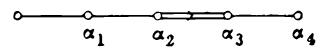
\includegraphics[keepaspectratio]{images/part002_560ef793.jpg}}

\begin{enumerate}
\def\labelenumi{(\Alph{enumi})}
\setcounter{enumi}{21}
\tightlist
\item
  \(R^{\prime}\) the set of vectors \(\pm2\varepsilon_{i},\pm\varepsilon_{i}\pm\varepsilon_{j},\pm\varepsilon_{1}\pm\varepsilon_{2}\pm\varepsilon_{3}\pm\varepsilon_{4}.\)
\end{enumerate}

\[
  \Phi_ {\mathrm{R}} (x, y) = \frac {(x | y)}{18}, \quad \gamma (\mathrm{R}) = 2. 3 ^ {4}.
\]

\begin{enumerate}
\def\labelenumi{(\Roman{enumi})}
\setcounter{enumi}{5}
\tightlist
\item
  Fundamental weights:
\end{enumerate}

\[
\omega_ {1} = \varepsilon_ {1} + \varepsilon_ {2} = 2 \alpha_ {1} + 3 \alpha_ {2} + 4 \alpha_ {3} + 2 \alpha_ {4}
\]

\[
\omega_ {2} = 2 \varepsilon_ {1} + \varepsilon_ {2} + \varepsilon_ {3} = 3 \alpha_ {1} + 6 \alpha_ {2} + 8 \alpha_ {3} + 4 \alpha_ {4}
\]

\[
\omega_ {3} = \frac {1}{2} (3 \varepsilon_ {1} + \varepsilon_ {2} + \varepsilon_ {3} + \varepsilon_ {4}) = 2 \alpha_ {1} + 4 \alpha_ {2} + 6 \alpha_ {3} + 3 \alpha_ {4}
\]

\[
\omega_ {4} = \varepsilon_ {1} = \alpha_ {1} + 2 \alpha_ {2} + 3 \alpha_ {3} + 2 \alpha_ {4}.
\]

\begin{enumerate}
\def\labelenumi{(\Roman{enumi})}
\setcounter{enumi}{6}
\tightlist
\item
  Sum of the positive roots:
\end{enumerate}

\[
2 \rho = 11 \varepsilon_ {1} + 5 \varepsilon_ {2} + 3 \varepsilon_ {3} + \varepsilon_ {4} = 16 \alpha_ {1} + 30 \alpha_ {2} + 42 \alpha_ {3} + 22 \alpha_ {4}.
\]

\begin{enumerate}
\def\labelenumi{(\Roman{enumi})}
\setcounter{enumi}{7}
\tightlist
\item
  \(\mathrm{Q}(\mathrm{R}) = \bigoplus_{i=1}^{4} \mathbf{Z} \varepsilon_i + \mathbf{Z}\left(\frac{1}{2} \sum_{i=1}^{4} \varepsilon_i\right)\) .
\end{enumerate}

\(P(R) = Q(R).\)

Connection index: 1.

\begin{enumerate}
\def\labelenumi{(\Roman{enumi})}
\setcounter{enumi}{8}
\item
  Exponents: 1, 5, 7, 11.
\item
  and (XI) A(R) = W(R), \(w_{0} = -1\) .
\item
  Cartan matrix:
\end{enumerate}

\[
\left( \begin{array}{c c c c} 2 & - 1 & 0 & 0 \\ - 1 & 2 & - 2 & 0 \\ 0 & - 1 & 2 & - 1 \\ 0 & 0 & - 1 & 2 \end{array} \right)
\]

\specialchapter{\texorpdfstring{PLATE IX. SYSTEM OF TYPE \(\mathbf{G}_2\)}{PLATE IX. SYSTEM OF TYPE G\_2}}

\begin{enumerate}
\def\labelenumi{(\Roman{enumi})}
\tightlist
\item
  V is the hyperplane in \(E = R^{3}\) with equation \(\xi_{1} + \xi_{2} + \xi_{3} = 0\) . Roots:
\end{enumerate}

\[
\begin{array}{c} \pm (\varepsilon_ {1} - \varepsilon_ {2}), \quad \pm (\varepsilon_ {1} - \varepsilon_ {3}), \quad \pm (\varepsilon_ {2} - \varepsilon_ {3}), \quad \pm (2 \varepsilon_ {1} - \varepsilon_ {2} - \varepsilon_ {3}), \\ \pm (2 \varepsilon_ {2} - \varepsilon_ {1} - \varepsilon_ {3}), \quad \pm (2 \varepsilon_ {3} - \varepsilon_ {1} - \varepsilon_ {2}). \end{array}
\]

Number of roots: n = 12.

\begin{enumerate}
\def\labelenumi{(\Roman{enumi})}
\setcounter{enumi}{1}
\item
  Basis: \(\alpha_{1} = \varepsilon_{1} - \varepsilon_{2},\alpha_{2} = -2\varepsilon_{1} + \varepsilon_{2} + \varepsilon_{3}\) . Positive roots: \(\alpha_{1},\alpha_{1} + \alpha_{2},2\alpha_{1} + \alpha_{2},3\alpha_{1} + \alpha_{2},3\alpha_{1} + 2\alpha_{2}\) .
\item
  Coxeter number: h = 6.
\item
  Highest root: \(\tilde{\alpha} = -\varepsilon_1 - \varepsilon_2 + 2\varepsilon_3 = 3\alpha_1 + 2\alpha_2 = \omega_2\) . Completed Dynkin graph:
\end{enumerate}

\pandocbounded{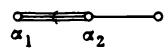
\includegraphics[keepaspectratio]{images/part002_d2921928.jpg}}

\begin{enumerate}
\def\labelenumi{(\Alph{enumi})}
\setcounter{enumi}{21}
\tightlist
\item
  \(R^{\prime}\) is the set of vectors
\end{enumerate}

\[
\pm \alpha_ {1}, \quad \pm (\alpha_ {1} + \alpha_ {2}), \quad \pm (2 \alpha_ {1} + \alpha_ {2}), \quad \pm \frac {1}{3} \alpha_ {2},
\]

\[
\pm \frac {1}{3} (3 \alpha_ {1} + \alpha_ {2}), \quad \pm \frac {1}{3} (3 \alpha_ {1} + 2 \alpha_ {2}).
\]

\[
  \Phi_ {\mathrm{R}} (x, y) = \frac {(x | y)}{24}, \quad \gamma (\mathrm{R}) = 48.
\]

\begin{enumerate}
\def\labelenumi{(\Roman{enumi})}
\setcounter{enumi}{5}
\tightlist
\item
  Fundamental weights:
\end{enumerate}

\[
\omega_ {1} = 2 \alpha_ {1} + \alpha_ {2}, \quad \omega_ {2} = 3 \alpha_ {1} + 2 \alpha_ {2} = \tilde {\alpha}.
\]

\begin{enumerate}
\def\labelenumi{(\Roman{enumi})}
\setcounter{enumi}{6}
\tightlist
\item
  Sum of the positive roots:
\end{enumerate}

\[
2 \rho = 2 (5 \alpha_ {1} + 3 \alpha_ {2}).
\]

\begin{enumerate}
\def\labelenumi{(\Roman{enumi})}
\setcounter{enumi}{7}
\item
  \(\mathrm{P}(\mathrm{R}) = \mathrm{Q}(\mathrm{R})\) . Connection index: 1.
\item
  Exponents: 1, 5.
\item
  W(R): the dihedral group of order 12.
\item
  and (XII): A(R) = W(R). \(w_{0} = -1\) .
\item
  Cartan matrix:
\end{enumerate}

\[
\left( \begin{array}{c c} 2 & - 1 \\ - 3 & 2 \end{array} \right)
\]

\specialchapter{PLATE X. IRREDUCIBLE SYSTEMS OF RANK 2}

\pandocbounded{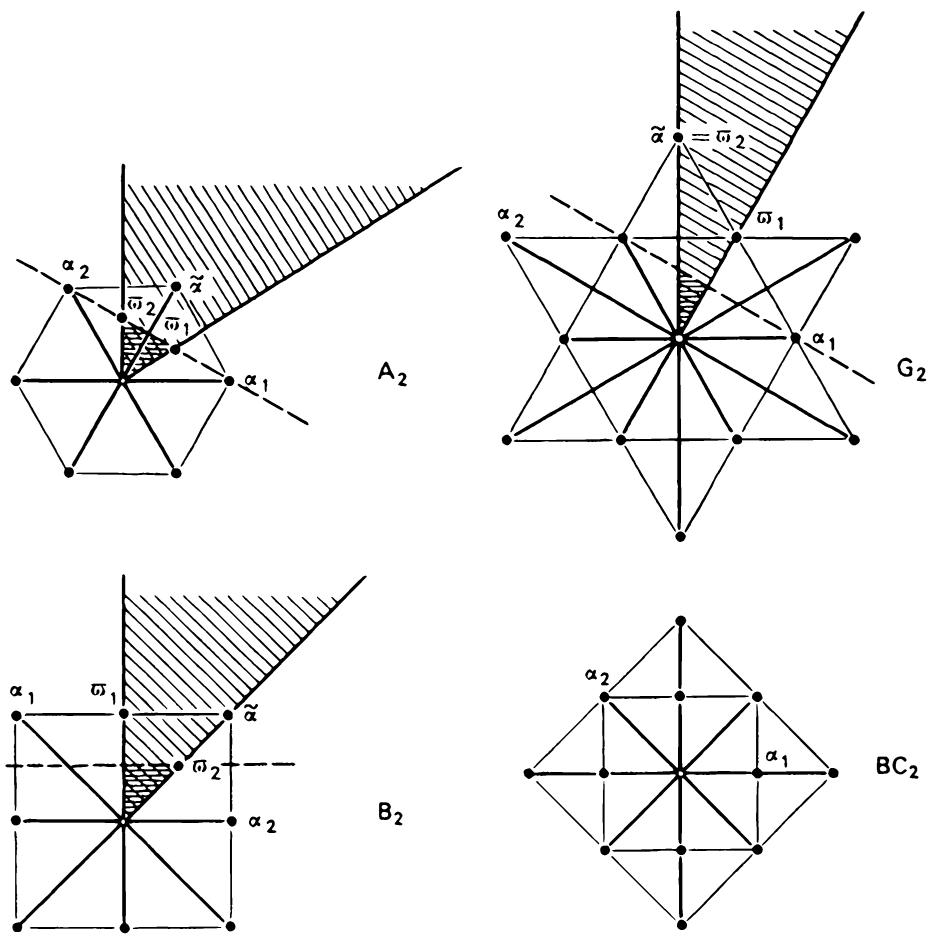
\includegraphics[keepaspectratio]{images/part002_e5dc67b9.jpg}}\\
The first three diagrams above represent the root systems R of type \(A_{2}\) . \(B_{2}\) and \(G_{2}\) . The shaded region represents the chamber C corresponding to the basis \((\alpha_{1},\alpha_{2})\) . The line \((x|\beta)=1\) , where \(\beta\) denotes the highest root of the

inverse system \(R^{-}\) , is shown dotted, and the doubly shaded region represents the alcove of \(R^{-}\) with vertex 0 contained in C.

The last diagram represents the unique irreducible non-reduced root system of rank 2.
